% !TEX root =../ECE343_Slides_Rogers.tex


\def\lessonNum{24}

%% pgffor
%\foreach \myl in {18,19,...,25}{
%	\ifnum\myl=\lessonNum
%		\includecomment{lesson\myl}
%		\message{YES lesson\myl}
%	\else
%		\excludecomment{lesson\myl}
%		\message{NO lesson\myl}
%	\fi
%}

%\forloop
%\newcounter{myc}
%\forloop{myc}{18}{\value{myc} < 25}{ %
%	\ifnum\value{myc}=\lessonNum
%		\includecomment{lesson\themyc}
%	\else
%		\excludecomment{lesson\themyc}
%	\fi
%} 

%
\ifnum\lessonNum=18
	\includecomment{lesson18}
	\excludecomment{lesson19}
	\excludecomment{lesson20}
	\excludecomment{lesson21}
	\excludecomment{lesson22}
	\excludecomment{lesson23}
	\excludecomment{lesson24}
	\excludecomment{lesson25}
\fi

\ifnum\lessonNum=19
	\excludecomment{lesson18}
	\includecomment{lesson19}
	\excludecomment{lesson20}
	\excludecomment{lesson21}
	\excludecomment{lesson22}
	\excludecomment{lesson23}
	\excludecomment{lesson24}
	\excludecomment{lesson25}
\fi

\ifnum\lessonNum=20
	\excludecomment{lesson18}
	\excludecomment{lesson19}
	\includecomment{lesson20}
	\excludecomment{lesson21}
	\excludecomment{lesson22}	
	\excludecomment{lesson23}
	\excludecomment{lesson24}
	\excludecomment{lesson25}
\fi

\ifnum\lessonNum=21
	\excludecomment{lesson18}
	\excludecomment{lesson19}
	\excludecomment{lesson20}
	\includecomment{lesson21}
	\excludecomment{lesson22}
	\excludecomment{lesson23}
	\excludecomment{lesson24}
	\excludecomment{lesson25}
\fi

\ifnum\lessonNum=22
	\excludecomment{lesson18}
	\excludecomment{lesson19}
	\excludecomment{lesson20}
	\excludecomment{lesson21}
	\includecomment{lesson22}
	\excludecomment{lesson23}
	\excludecomment{lesson24}
	\excludecomment{lesson25}
\fi

\ifnum\lessonNum=23
	\excludecomment{lesson18}
	\excludecomment{lesson19}
	\excludecomment{lesson20}
	\excludecomment{lesson21}
	\excludecomment{lesson22}
	\includecomment{lesson23}
	\excludecomment{lesson24}
	\excludecomment{lesson25}
\fi

\ifnum\lessonNum=24
	\excludecomment{lesson18}
	\excludecomment{lesson19}
	\excludecomment{lesson20}
	\excludecomment{lesson21}
	\excludecomment{lesson22}
	\excludecomment{lesson23}
	\includecomment{lesson24}
	\excludecomment{lesson25}
\fi

\ifnum\lessonNum=25
	\excludecomment{lesson18}
	\excludecomment{lesson19}
	\excludecomment{lesson20}
	\excludecomment{lesson21}
	\excludecomment{lesson22}
	\excludecomment{lesson23}
	\excludecomment{lesson24}
	\includecomment{lesson25}
\fi

%\begin{comment}
\section{Schedule}
\renewcommand{\arraystretch}{1}
\begin{frame}{}
	\begin{textblock}{14}(0.5,1.75)
	\def\myfontsize{footnotesize}
	\input{./Schedule_Prog}
	\end{textblock}
\end{frame}

%%%%%%%%%%%%%%%%%%%%%%%%%%%%%%%%%%%%%%%%%%%%%%%%%%%%%%%%%%%%%%%%%%
%%%%%%%%%%%%%%%%%%%%%%%%%%%%%%%%%%%%%%%%%%%%%%%%%%%%%%%%%%%%%%%%%%

\begin{frame}{}
\renewcommand{\arraystretch}{1}
	\begin{textblock}{14}(0.5,1.75)
	\def\myfontsize{footnotesize}
	\input{./Schedule_Final}
	\end{textblock}
\end{frame}


%%%%%%%%%%%%%%%%%%%%%%%%%%%%%%%%%%%%%%%%%%%%%%%%%%%%%
%%%%%%%%%%%%%%%%%%%%%%%%%%%%%%%%%%%%%%%%%%%%%%%%%%%%%

\begin{frame}{Learning Objectives}
	\begin{textblock}{14}(0.5,4)
	\begin{enumerate}[{3}.1]
		\item Apply Coloumb's Law to use direct integration to calculate the electric field due to charge density in varoius geometries, including rectangular, cylindrical, and spherical coordinate systems. 
		\item Apply the integral and differential forms of Gauss' Law to calculate the electric field due to charge density in various geometries, including rectangular, cylindrical, and spherical coordinate systems. 
		\item Calculate the electric field from the scalar electric potential in a variety of geometries.
		\item  Apply the electric field boundary conditions to calculate electric fields on both sides of a material boundary. 
	\end{enumerate}
	\end{textblock}
\end{frame}

\begin{lesson18}
%%%%%%%%%%%%%%%%%%%%%%%%%%%%%%%%%%%%%%%%%%%%%%%%%%%%%%
%%%%%%%%%%%%%%%%%%%%%%%%%%%%%%%%%%%%%%%%%%%%%%%%%%%%%%
\begin{frame}{Coloumb Force}
\begin{textblock}{7}(0.5,3)
\begin{tikzpicture}[scale=0.7]
		\def\qonex{0}
		\def\qoney{3}
		\def\qtwox{0}
		\def\qtwoy{-2}
		\def\qthreex{4}
		\def\qthreey{0}
		\begin{axis}[ 
		domain=-5:5,
%		samples=200, 
%		xmin=-1, 
		xmax=4.5, 
		ymax=4,
		ymin=-4,
%		title={Single Square Pulse, $\Pi (\frac{t}{\tau})$},
%		scaled x ticks=base 10:6,
%		xtick scale label code/.code={},
%		minor x tick num = 5,
%		minor y tick num = 5,
%		ytick={-1,0,1},
%		xtick={-5,-4,-3,-2,-1,0,1,2,3,4,5},
%		xticklabels={$-\frac{\tau}{2}$,$\frac{\tau}{2}$},
		xlabel={$\rho$},
		ylabel={$z$},
		axis y line = middle,
		axis x line = middle,
		x label style={xshift=-0.5cm},
		x label style={yshift=-1cm},
		y label style ={xshift=-1.25cm},
%		y label style = {yshift =1cm},
		clip=false,
		]
		\addplot [mark=*] coordinates  {(\qonex,\qoney)} node[right, xshift=0.35cm] {$q_1 = -3\mu$C};
		\addplot [mark=*] coordinates  {(\qtwox,\qtwoy)} node[right, xshift=0.35cm] {$q_2 = 1\mu$C};
		\addplot [mark=*] coordinates  {(\qthreex,\qthreey)} node[above, yshift=0.25cm] {$q_3 =2\mu$C};
		\addplot[dashed, decoration={markings,mark=at position 0.8 with {\arrow[scale=3]{stealth}}}, postaction={decorate}] coordinates {(\qonex,\qoney)(\qthreex,\qthreey)};
		\addplot[dashed, decoration={markings,mark=at position 0.8 with {\arrow[scale=3]{stealth}}}, postaction={decorate}] coordinates {(\qtwox,\qtwoy)(\qthreex,\qthreey)};
		\end{axis}
\end{tikzpicture}

	\eq{
		&\vec{F}_{mn} = \dfrac{q_m q_n }{4\pi | R|^2} \hat{R} =  \dfrac{q_m q_n }{4\pi | R|^3} \vec{R} \\ 
		&\text{ with: } \vec{R} = \vec{r} - \vec{r}^{\;\prime} \\
	}
\end{textblock}
\begin{textblock}{8}(7.5,3)
\visible<0|handout:1>{
\begin{scriptsize}
\alert{
	\eq{
		\vec{F}_3 &= \vec{F}_{31} + \vec{F}_{32} \\
		\vec{R} &= \lp \xhat 4 + \yhat 0 \rp - \lp \xhat 0 + \yhat 3 \rp  = \xhat 4 - \yhat 3 \\
		\vec{F}_{31} &= \dfrac{\lp-3\mu\text{C}\rp\lp 2\mu\text{C}\rp}{\lp 4\pi \rp \lp 8.854\ee{-12} \rp \lp \sqrt{25}\rp^3}	\lp \xhat 4 - \yhat 3 \rp \\
		&= \lp-1.724\xhat + 1.293\yhat \rp \text{mN}\\
		\vec{F}_{32} &= \dfrac{\lp 1\mu\text{C}\rp\lp 2\mu\text{C}\rp}{\lp 4\pi \rp \lp 8.854\ee{-12} \rp \lp \sqrt{20}\rp^3}	\lp \xhat 4 + \yhat 2 \rp \\
		&= \lp 0.8\xhat + 0.4\yhat \rp\text{mN} \\
		&\implies \vec{F}_3 = \lp -0.9\xhat + 1.69\yhat \rp \text{mN}
	} % end eq
} % end alert
\end{scriptsize}
} % end visible 
\end{textblock}
\end{frame}

%%%%%%%%%%%%%%%%%%%%%%%%%%%%%%%%%%%%%%%%%%%%%%%%%%%%%%
%%%%%%%%%%%%%%%%%%%%%%%%%%%%%%%%%%%%%%%%%%%%%%%%%%%%%%
\begin{frame}{$\vec{E}$ by Direct Integration: Line Charge}
\begin{textblock}{7}(0.5,3)
\begin{tikzpicture}[scale=0.7]
		\def\qonex{0}
		\def\qoney{3}
		\def\qtwox{0}
		\def\qtwoy{-2}
		\def\qthreex{4}
		\def\qthreey{0}
		\begin{axis}[ 
		domain=-5:5,
%		samples=200, 
%		xmin=-1, 
		xmax=4.5, 
		ymax=3.5,
		ymin=-2.5,
%		title={Single Square Pulse, $\Pi (\frac{t}{\tau})$},
%		scaled x ticks=base 10:6,
%		xtick scale label code/.code={},
%		minor x tick num = 5,
%		minor y tick num = 5,
%		ytick={-1,0,1},
%		xtick={-5,-4,-3,-2,-1,0,1,2,3,4,5},
%		xticklabels={$-\frac{\tau}{2}$,$\frac{\tau}{2}$},
		xlabel={$\rho$},
		ylabel={$z$},
		axis y line = middle,
		axis x line = middle,
		x label style={xshift=0.5cm},
		x label style={yshift=-0.25cm},
		y label style ={xshift=-0.25cm},
		y label style = {yshift =0.5cm},
		clip=false,
		]
		\addplot [mark=*] coordinates  {(\qonex,\qoney)} node[right, xshift=0.35cm] {$dq$};
		\addplot [mark=*] coordinates  {(\qthreex,\qthreey)} node[above, yshift=0.25cm] {$q_3$};
		\addplot[dashed, decoration={markings,mark=at position 0.8 with {\arrow[scale=3]{stealth}}}, postaction={decorate}] coordinates {(\qonex,\qoney)(\qthreex,\qthreey)};
		\addplot[thick, red] coordinates {(0,-3.5)(0,3.5)};
		\node at (-0.5,-3.5) {$-\dfrac{L}{2}$};
		\node at (-0.5,3.5) {$\dfrac{L}{2}$};
		\end{axis}
\end{tikzpicture}

\end{textblock}
\begin{textblock}{8}(7.5,3)
\begin{myblock}[0.9]{Method}
\begin{enumerate}
	\item Draw picture 
	\item Write ``Coulomb's Law'':
		\eq{
			d\vec{E} = \dfrac{dQ}{4\pi \varepsilon | R |^3}\vec{R}
		}
	\item Define $dQ$ in terms of charge distribution ($\rho$) and length ($d\ell$)
	\item Define $\vec{R}$ 
	\item Integrate to find $\vec{E}$
\end{enumerate}
\end{myblock}
\end{textblock}

\end{frame}

\end{lesson18}

%%%%%%%%%%%%%%%%%%%%%%%%%%%%%%%%%%%%%%%%%%%%%%%%%%%%%%%%%%%%
%%%%%%%%%%%%%%%%%%%%%%%%%%%%%%%%%%%%%%%%%%%%%%%%%%%%%%%%%%%%

\begin{lesson19}

\begin{frame}{$\vec{E}$ by Direct Integration: Line Charge}
\begin{textblock}{7}(0.5,3)
\begin{tikzpicture}[scale=0.7]
		\def\qonex{0}
		\def\qoney{3}
		\def\qtwox{0}
		\def\qtwoy{-2}
		\def\qthreex{4}
		\def\qthreey{0}
		\begin{axis}[ 
		domain=-5:5,
%		samples=200, 
%		xmin=-1, 
		xmax=4.5, 
		ymax=3.5,
		ymin=-3.5,
%		title={Single Square Pulse, $\Pi (\frac{t}{\tau})$},
%		scaled x ticks=base 10:6,
%		xtick scale label code/.code={},
%		minor x tick num = 5,
%		minor y tick num = 5,
		ytick={-3,3},
		yticklabels={$-\dfrac{L}{2}$, $\dfrac{L}{2}$},
		xtick=\empty,
%		xticklabels={$\rho$},
		xlabel={$\rho$},
		ylabel={$z$},
		axis y line = middle,
		axis x line = middle,
		x label style={xshift=0.5cm},
		x label style={yshift=-0.25cm},
		y label style ={xshift=-0.25cm},
		y label style = {yshift =0.5cm},
		clip=false,
		]
		\addplot [mark=*] coordinates  {(\qonex,\qoney)} node[right, xshift=0.35cm] {$dq$};
		\addplot [mark=*] coordinates  {(\qthreex,\qthreey)} node[above, yshift=0.25cm] {Observer};
		\addplot[dashed, decoration={markings,mark=at position 0.8 with {\arrow[scale=3]{stealth}}}, postaction={decorate}] coordinates {(\qonex,\qoney)(\qthreex,\qthreey)};
		\addplot[thick, red] coordinates {(0,-3.5)(0,3.5)};
		\node[red] at (-0.5,0) {$\rho_L$};
		\end{axis}
\end{tikzpicture}
%\alert{
%\begin{scriptsize}
%	\eq{
%		d\vec{E} &= \dfrac{dQ}{\lp 4\pi \varepsilon \rp |R|^3 } \vec{R} \\ 
%		dQ &= \rho_L dz \\
%		\vec{R} & = \rhohat \rho - \zhat z 
%		}
%\end{scriptsize}
%} % end alert
\end{textblock}
%\begin{textblock}{8}(7.75,3.5)
%\visible<0|handout:1>{
%\begin{scriptsize}
%\alert{
%	\eq{
%		d\vec{E} &= \dfrac{dQ}{\lp 4\pi \varepsilon \rp |R|^3 } \vec{R} \\ 
%		dQ &= \rho_L dz \\
%		\vec{R} & = \rhohat \rho - \zhat z \\
%		\vec{E} &= \int \dfrac{\rho_L dz }{\lp 4\pi \varepsilon \rp \lp\sqrt{\rho^2 + z^2 } \rp^3 } \lp \rhohat \rho - \zhat z \rp \\
%		&=  \int\rhohat\dfrac{\rho_L  \rho}{\lp 4\pi \varepsilon \rp \lp\rho^2 + z^2 \rp^{3/2} } dz \\
%		 & - \int\zhat\dfrac{\rho_L  z }{\lp 4\pi \varepsilon \rp \lp\rho^2 + z^2 \rp^{3/2} } dz  
%	} % end eq
%} % end alert
%\end{scriptsize}
%} % end visible 
%\end{textblock}
%
%\end{frame}

\begin{textblock}{8}(8,2.75)
\begin{myblock}[0.9]{Method}
	\begin{enumerate}
		\setlength\itemsep{12pt}
		\item Draw picture 
		\item Write ``Coulomb's Law'':
			
			\vspace{-18pt}
			\eq{
				d\vec{E} = \dfrac{dQ}{4\pi \varepsilon | R |^3}\vec{R}
			}
			\vspace{-28pt}
			
		\item Define $dQ = \handoutgap{0pt}{\rho_\ell d\ell = \rho_L dz} $ 
		\item Define $\vec{R} = \handoutgap{0pt}{ \rhohat \rho - \zhat z } $ 
		\vspace{-8pt}
		\eq{
			d\vec{E} &= \handoutgap{1in}{\dfrac{\rho_L dz }{\lp 4\pi \varepsilon \rp \lp\sqrt{\rho^2 + z^2 } \rp^3 }  } \\
					&\handoutgap{0in}{\qquad\lp \rhohat \rho - \zhat z \rp}
			}
		
	\end{enumerate}
\end{myblock}
\end{textblock}
\end{frame}
%%%%%%%%%%%%%%%%%%%%%%%%%%%%%%%%%%%%%%%%%%%%%%%%%%%%%%
%%%%%%%%%%%%%%%%%%%%%%%%%%%%%%%%%%%%%%%%%%%%%%%%%%%%%%


\begin{frame}{$\vec{E}$ by Direct Integration: Line Charge}
\begin{textblock}{7}(0.5,3)
\visible<0|handout:1>{
\begin{scriptsize}
\alert{
\rhohat$\;$ component:
\eq{
	 &\implies \rhohat \dfrac{\rho_L \rho}{4\pi \varepsilon} \int^{L/2}_{-L/2} \dfrac{1}{ \lp\rho^2 + z^2 \rp^{3/2} } dz \\
		 &\implies \rhohat \dfrac{\rho_L \rho}{4\pi \varepsilon} \lp \dfrac{z}{\rho^2 \sqrt{\rho^2 + z^2}} \rp\Bigg|^{L/2}_{-L/2} \\
		 & = \rhohat \dfrac{\rho_L \rho}{4\pi \varepsilon} \lp \dfrac{\dfrac{L}{2}}{\rho^2 \sqrt{\rho^2 + \lp\dfrac{L}{2}\rp^2}} - \dfrac{-\dfrac{L}{2}}{\rho^2 \sqrt{\rho^2 + \lp-\dfrac{L}{2}\rp^2}} \rp \\
		 & = \rhohat \dfrac{\rho_L \rho}{4\pi \varepsilon} \lp \dfrac{L}{\rho^2 \sqrt{\rho^2 + \lp\dfrac{L}{2}\rp^2}} \rp \\
		 &= \rhohat \dfrac{\rho_L L }{4\pi \varepsilon\rho\sqrt{\rho^2 + \lp\dfrac{L}{2}\rp^2}} 
	} % end eq
} % end alert
\end{scriptsize}
} % end visible 
\end{textblock}

\begin{textblock}{8}(8.5,3)
\visible<0|handout:1>{
\begin{scriptsize}
\alert{
\zhat$\;$ component:
\eq{
	&\implies -\zhat \dfrac{\rho_L}{4\pi\varepsilon} \int^{L/2}_{-L/2} \dfrac{z}{ \lp\rho^2 + z^2 \rp^{3/2} } dz \\
	&\implies   -\zhat \dfrac{\rho_L}{4\pi\varepsilon} \lp \dfrac{1}{\sqrt{\rho^2 + z^2}} \rp\Bigg|^{L/2}_{-L/2} \\
	&=  -\zhat \dfrac{\rho_L}{4\pi\varepsilon} \lp\dfrac{1}{\sqrt{\rho^2 +\lp\dfrac{L}{2}\rp^2}}\right.\\
	& \qquad \left. - \dfrac{1}{\sqrt{\rho^2 +\lp-\dfrac{L}{2}\rp^2}} \rp \\
	&= 0
}
} % end alert
\end{scriptsize}
} % end visible 
\end{textblock}
\end{frame}

%%%%%%%%%%%%%%%%%%%%%%%%%%%%%%%%%%%%%%%%%%%%%%%%%%%%%%
%%%%%%%%%%%%%%%%%%%%%%%%%%%%%%%%%%%%%%%%%%%%%%%%%%%%%%
\begin{frame}{$\vec{E}$ by Direct Integration: Line Charge}
\begin{textblock}{7}(0.5,3)
\begin{tikzpicture}[scale=0.7]
		\def\qonex{0}
		\def\qoney{3}
		\def\qtwox{0}
		\def\qtwoy{-2}
		\def\qthreex{4}
		\def\qthreey{0}
		\begin{axis}[ 
		domain=-5:5,
%		samples=200, 
%		xmin=-1, 
		xmax=4.5, 
		ymax=3.5,
		ymin=-3.5,
%		title={Single Square Pulse, $\Pi (\frac{t}{\tau})$},
%		scaled x ticks=base 10:6,
%		xtick scale label code/.code={},
%		minor x tick num = 5,
%		minor y tick num = 5,
		ytick={-3,3},
		yticklabels={$-\dfrac{L}{2}$, $\dfrac{L}{2}$},
		xtick=\empty,
%		xticklabels={$\rho$},
		xlabel={$\rho$},
		ylabel={$z$},
		axis y line = middle,
		axis x line = middle,
		x label style={xshift=0.5cm},
		x label style={yshift=-0.25cm},
		y label style ={xshift=-0.25cm},
		y label style = {yshift =0.5cm},
		clip=false,
		]
		\addplot [mark=*] coordinates  {(\qonex,\qoney)} node[right, xshift=0.35cm] {$dq$};
		\addplot [mark=*] coordinates  {(\qthreex,\qthreey)} node[above, yshift=0.25cm] {Observer};
		\addplot[dashed, decoration={markings,mark=at position 0.8 with {\arrow[scale=3]{stealth}}}, postaction={decorate}] coordinates {(\qonex,\qoney)(\qthreex,\qthreey)};
		\addplot[thick, red] coordinates {(0,-3.5)(0,3.5)};
		\node[red] at (-0.5,0) {$\rho_L$};
		\end{axis}
\end{tikzpicture}

\end{textblock}
\begin{textblock}{8}(7.75,2.5)
\begin{myblock}[0.9]{Result}
	\eq{
		\vec{E} =  \rhohat \dfrac{\rho_L L }{4\pi \varepsilon\rho\sqrt{\rho^2 + \lp\frac{L}{2}\rp^2}} 
	} % end eq
\end{myblock}

\begin{myblock}[0.9]{Infinite Wire Approx}
For $\dfrac{L}{2} >> \rho$:
	\eq{
		\vec{E} &=  \rhohat \dfrac{\rho_L L }{4\pi \varepsilon\rho\sqrt{\lp\frac{L}{2}\rp^2}} 
				= \dfrac{\rho_L}{2\pi \varepsilon \rho}
	} % end eq
\end{myblock}
\end{textblock}

\end{frame}

%%%%%%%%%%%%%%%%%%%%%%%%%%%%%%%%%%%%%%%%%%%%%%%%%%%%%%
%%%%%%%%%%%%%%%%%%%%%%%%%%%%%%%%%%%%%%%%%%%%%%%%%%%%%%

\begin{frame}{Wire Loop: Direct Integration}
\begin{textblock}{7}(0.5,3)
Find the Electric field at $z=h$ from a line charge carrying a charge distribution of $\rho_\ell$. 
\tdplotsetmaincoords{70}{110}
	\begin{tikzpicture}[tdplot_main_coords]
	
		\coordinate (O) at (0,0,0);
		\draw[thick, <->] (-3.5,0,0) -- (3.5,0,0) node[anchor=north east]{$x$};
		\draw[thick,<->] (0,-2.5,0) --(0,3,0) node[anchor=north west]{$y$}; 
		\draw[thick,->] (0,0,0) --(0,0,3) node[anchor=south]{$z$}; 
	
	\tdplotdrawarc[blue]{(O)}{2}{0}{360}{anchor=north}{}
	\tdplotdrawarc[->]{(O)}{0.75}{0}{45}{anchor=north}{$\phi$}
	\draw[red] (0,0,0) to (-1.4,1.4,0) node[above left, midway] {$a$};
	\draw[fill=black] (0,0,2) circle (2pt); 
	\node at (0,0.75,2) {$h$};
	\node at (2,2,0) {$\rho_\ell$};
	\end{tikzpicture}
\end{textblock}
\begin{textblock}{8}(8,2.75)
\begin{myblock}[0.9]{Method}
	\begin{enumerate}
		\setlength\itemsep{12pt}
		\item Draw picture 
		\item Write ``Coulomb's Law'':
			
			\vspace{-18pt}
			\eq{
				d\vec{E} = \dfrac{dQ}{4\pi \varepsilon | R |^3}\vec{R}
			}
			\vspace{-28pt}
			
		\item Define $dQ = \handoutgap{0pt}{\rho_\ell d\ell = \rho_\ell a d\phi} $ 
		\item Define $\vec{R} = \handoutgap{0pt}{-a\rhohat + h\zhat} $ 
		\vspace{-12pt}
		\eq{
			d\vec{E} &= \handoutgap{1in}{\dfrac{\rho_\ell a}{4\pi \varepsilon \lp a^2 + h^2 \rp^{3/2}} } \\
					&\handoutgap{0in}{\qquad\lp -a\rhohat + h\zhat \rp d\phi}
			}
		
	\end{enumerate}
\end{myblock}
\end{textblock}

\end{frame}

%%%%%%%%%%%%%%%%%%%%%%%%%%%%%%%%%%%%%%%%%%%%%%%%%%%%%%
%%%%%%%%%%%%%%%%%%%%%%%%%%%%%%%%%%%%%%%%%%%%%%%%%%%%%%

\begin{frame}{Wire Loop: Direct Integration (cont'd)}
\begin{textblock}{7}(0.5,3)
\visible<0|handout:1>{
\begin{scriptsize}
\alert{
\rhohat$\;$ component:
\eq{
	 &\implies \int^{2\pi}_{0} \rhohat \dfrac{\rho_\ell a^2 }{4\pi \varepsilon \lp a^2 + h^2 \rp^{3/2}}d\phi  \\
	&\implies 	 \dfrac{\rho_\ell a^2 }{4\pi \varepsilon \lp a^2 + h^2 \rp^{3/2}}\int^{2\pi}_{0} \rhohat d\phi \\
	&\text{...but } \rhohat = \xhat\cosp{\phi} + \yhat\sinp{\phi} \\
	&\implies \dfrac{\rho_\ell a^2 }{4\pi \varepsilon \lp a^2 + h^2 \rp^{3/2}}\int^{2\pi}_{0}  \xhat\cosp{\phi} + \yhat\sinp{\phi} d\phi \\
	&\implies \dfrac{\rho_\ell a^2 }{4\pi \varepsilon \lp a^2 + h^2 \rp^{3/2}} \lp 0 + 0  \rp
	} % end eq
} % end alert
\end{scriptsize}
} % end visible 
\end{textblock}

\begin{textblock}{8}(8.5,3)
\visible<0|handout:1>{
\begin{scriptsize}
\alert{
\zhat$\;$ component:
\eq{
	 &\implies \int^{2\pi}_{0} \zhat \dfrac{\rho_\ell ah }{4\pi \varepsilon \lp a^2 + h^2 \rp^{3/2}}d\phi  \\
	 &\implies \zhat\dfrac{\rho_\ell ah }{4\pi \varepsilon \lp a^2 + h^2 \rp^{3/2}} \int^{2\pi}_{0}  d\phi \\
	 &\implies \zhat \dfrac{\rho_\ell ah }{2 \varepsilon \lp a^2 + h^2 \rp^{3/2}}
}
} % end alert
\end{scriptsize}
} % end visible 
\end{textblock}

\begin{textblock}{14.5}(0.5,11)
\begin{myblock}[0.9]{Result}
	\vspace{-12pt}
	\eq{
		\vec{E} &= \handoutgap{0pt}{ \zhat \dfrac{\rho_\ell ah }{2 \varepsilon \lp a^2 + h^2 \rp^{3/2}} }
	}
\end{myblock}
\end{textblock}
\end{frame}


%%%%%%%%%%%%%%%%%%%%%%%%%%%%%%%%%%%%%%%%%%%%%%%%%%%%%%%%%%%%
%%%%%%%%%%%%%%%%%%%%%%%%%%%%%%%%%%%%%%%%%%%%%%%%%%%%%%%%%%%%

\begin{frame}{Partial Line: Direct Integration}
\begin{textblock}{7}(0.5,3)
Find the Electric field at $z=h$ from a partial loop carrying a charge distribution of $\rho_\ell$. 
\tdplotsetmaincoords{70}{110}
	\begin{tikzpicture}[tdplot_main_coords]
	
		\coordinate (O) at (0,0,0);
		\draw[thick, <->] (-3.5,0,0) -- (3.5,0,0) node[anchor=north east]{$x$};
		\draw[thick,<->] (0,-2.5,0) --(0,3,0) node[anchor=north west]{$y$}; 
		\draw[thick,->] (0,0,0) --(0,0,3) node[anchor=south]{$z$}; 
	
	\tdplotdrawarc[blue]{(O)}{2}{0}{90}{anchor=north}{}
	\tdplotdrawarc[->]{(O)}{0.75}{0}{45}{anchor=north}{$\phi$}
	\draw[red] (0,0,0) to (1.4,1.4,0) node[above left, midway] {$a$};
	\draw[fill=black] (0,0,2) circle (2pt); 
	\node at (0,0.75,2) {$h$};
	\node at (2,2,0) {$\rho_\ell$};
	\end{tikzpicture}
\end{textblock}
\begin{textblock}{8}(8,3)
\begin{myblock}[0.9]{Method}
	\begin{enumerate}
		\setlength\itemsep{12pt}
		\item Draw picture 
		\item Write ``Coulomb's Law'':
			
			\vspace{-18pt}
			\eq{
				d\vec{E} = \dfrac{dQ}{4\pi \varepsilon | R |^3}\vec{R}
			}
			\vspace{-28pt}
			
		\item Define $dQ = \handoutgap{0pt}{\rho_\ell \rho d\phi = \rho_\ell a d\phi} $ 
		\item Define $\vec{R} = \handoutgap{0pt}{-a\rhohat + h\zhat} $ 
		\vspace{-12pt}
		\eq{
			d\vec{E} &= \handoutgap{1in}{\dfrac{\rho_\ell a }{4\pi \varepsilon \lp a^2 + h^2 \rp^{3/2}} } \\
					&\handoutgap{0in}{\qquad\lp -a\rhohat + h\zhat \rp d\phi}
			}
		
	\end{enumerate}
\end{myblock}
\end{textblock}

\end{frame}

%%%%%%%%%%%%%%%%%%%%%%%%%%%%%%%%%%%%%%%%%%%%%%%%%%%%%%%%%%%%
%%%%%%%%%%%%%%%%%%%%%%%%%%%%%%%%%%%%%%%%%%%%%%%%%%%%%%%%%%%%

\begin{frame}{Partial Line: Direct Integration}
\begin{textblock}{7}(0.5,3)
\visible<0|handout:1>{
\begin{scriptsize}
\alert{
\rhohat$\;$ component:
\eq{
	 &\implies \int^{\pi/2}_{0} \rhohat \dfrac{\rho_\ell a^2 }{4\pi \varepsilon \lp a^2 + h^2 \rp^{3/2}}d\phi  \\
	&\implies 	 \dfrac{\rho_\ell a^2 }{4\pi \varepsilon \lp a^2 + h^2 \rp^{3/2}}\int^{\pi/2}_{0} \rhohat d\phi \\
	&\text{...but } \rhohat = \xhat\cosp{\phi} + \yhat\sinp{\phi} \\
	&\implies \dfrac{\rho_\ell a^2 }{4\pi \varepsilon \lp a^2 + h^2 \rp^{3/2}}\int^{\pi/2}_{0}  \xhat \cosp{\phi} + \yhat\sinp{\phi} d\phi \\
	&\implies \dfrac{\rho_\ell a}{4\pi \varepsilon \lp a^2 + h^2 \rp^{3/2}} \lp -\xhat a -\yhat a  \rp
	} % end eq
} % end alert
\end{scriptsize}
} % end visible 
\end{textblock}

\begin{textblock}{8}(8.5,3)
\visible<0|handout:1>{
\begin{scriptsize}
\alert{
\zhat$\;$ component:
\eq{
	 &\implies \int^{\pi/2}_{0} \zhat \dfrac{\rho_\ell ah }{4\pi \varepsilon \lp a^2 + h^2 \rp^{3/2}}d\phi  \\
	 &\implies \zhat\dfrac{\rho_\ell a }{4\pi \varepsilon \lp a^2 + h^2 \rp^{3/2}} \int^{\pi/2}_{0}  h d\phi \\
	 &\implies \zhat \dfrac{\rho_\ell a }{4\pi\varepsilon \lp a^2 + h^2 \rp^{3/2}} \lp \dfrac{h\pi}{2}\rp 
}
} % end alert
\end{scriptsize}
} % end visible 
\end{textblock}

\begin{textblock}{14.5}(0.5,11)
\begin{myblock}[0.9]{Result}
	\vspace{-12pt}
	\eq{
		\vec{E} &= \handoutgap{0pt}{ \dfrac{\rho_\ell a}{4\pi \varepsilon \lp a^2 + h^2 \rp^{3/2}} \lp -\xhat a -\yhat a   + \zhat \dfrac{h\pi}{2} \rp}
	}
\end{myblock}
\end{textblock}
\end{frame}

%%%%%%%%%%%%%%%%%%%%%%%%%%%%%%%%%%%%%%%%%%%%%%%%%%%%%%%%%%%%
%%%%%%%%%%%%%%%%%%%%%%%%%%%%%%%%%%%%%%%%%%%%%%%%%%%%%%%%%%%%

\begin{frame}{Disk Charge: Direct Integration}
\begin{textblock}{7}(0.5,3)
Find the Electric field at $z=h$ from a disk carrying a charge distribution of $\rho_S$. 
\tdplotsetmaincoords{70}{110}
	\begin{tikzpicture}[tdplot_main_coords]
	
		\coordinate (O) at (0,0,0);
		\draw[thick, <->] (-3.5,0,0) -- (3.5,0,0) node[anchor=north east]{$x$};
		\draw[thick,<->] (0,-2.5,0) --(0,3,0) node[anchor=north west]{$y$}; 
		\draw[thick,->] (0,0,0) --(0,0,3) node[anchor=south]{$z$}; 
	
	\tdplotdrawarc[blue]{(O)}{2}{0}{360}{anchor=north}{}
	\tdplotdrawarc[->]{(O)}{0.75}{0}{45}{anchor=north}{$\phi$}
	%\draw[,blue,->] (1.4,-1.4) to (-0.1,-0.1,1.9) node[above left] {};
	\draw[fill=black] (0,0,2) circle (2pt); 
	\node at (0,0.75,2) {$h$};
	\node[blue] at (-1,1,0) {$\rho_S (\text{\footnotesize{C/m}}^2)$};
	\end{tikzpicture}
\end{textblock}
\begin{textblock}{8}(8,3)
\begin{myblock}[0.9]{Method}
	\begin{enumerate}
		\setlength\itemsep{12pt}
		\item Draw picture 
		\item Write ``Coulomb's Law'':
			
			\vspace{-18pt}
			\eq{
				d\vec{E} = \dfrac{dQ}{4\pi \varepsilon | R |^3}\vec{R}
			}
			\vspace{-28pt}
			
		\item Define $dQ = \handoutgap{0pt}{\rho_S \rho d\rho d\phi } $ 
		\item Define $\vec{R} = \handoutgap{0pt}{-\rho\rhohat + h\zhat} $ 
		\vspace{-12pt}
		\eq{
			d\vec{E} &= \handoutgap{1in}{\dfrac{\rho_S \rho }{4\pi \varepsilon \lp \rho^2 + h^2 \rp^{3/2}} } \\
					&\handoutgap{0in}{\qquad\lp -\rho\rhohat + h\zhat \rp d\rho d\phi}
			}
		
	\end{enumerate}
\end{myblock}
\end{textblock}

\end{frame}

%%%%%%%%%%%%%%%%%%%%%%%%%%%%%%%%%%%%%%%%%%%%%%%%%%%%%%
%%%%%%%%%%%%%%%%%%%%%%%%%%%%%%%%%%%%%%%%%%%%%%%%%%%%%%
\begin{frame}{Disk Charge: Direct Integration (cont'd)}
\begin{textblock}{14.5}(0.5,3)
6. Integrate to find $\vec{E}$:

\vspace{-12pt}
\visible<0|handout:1>{
\begin{scriptsize}
	\alert{
		\eq{
			\rhohat \text{ component } &\longrightarrow 0 \\
			\zhat \text{ component } &\longrightarrow  \zhat \dfrac{\rho_S h}{4\pi\varepsilon}\int_0^{2\pi} \int_{0}^{a} \dfrac{\rho}{\lp \rho^2 + h^2 \rp^{3/2}} d\rho d\phi  \qquad
			= \zhat \dfrac{\rho_S h}{4\pi\varepsilon}\int_0^{2\pi} d\phi \int_{0}^{a} \dfrac{\rho}{\lp \rho^2 + h^2 \rp^{3/2}} d\rho  \\
			&= \zhat \dfrac{2\pi\rho_S h}{4\pi\varepsilon} \int_{0}^{a} \dfrac{\rho}{\lp \rho^2 + h^2 \rp^{3/2}} d\rho \qquad
			=\zhat \dfrac{\rho_S h}{2\varepsilon} \int_{0}^{a} \dfrac{\rho}{\lp \rho^2 + h^2 \rp^{3/2}} d\rho \\
			u &= \rho^2 + h^2 \qquad du = 2\rho d\rho  \implies \dfrac{1}{2}\int u^{-3/2} du 
			= -u^{-1/2}  \longrightarrow -\dfrac{1}{\sqrt{\rho^2 + h^2}}\\
			&\implies  -\zhat \dfrac{\rho_S h}{2\varepsilon \sqrt{\rho^2 + h^2}} \Bigg|_{\rho=0}^{a} \qquad
			 = \zhat \dfrac{\rho_S h}{2\varepsilon \sqrt{\rho^2 + h^2}} \lp -\dfrac{1}{\sqrt{a^2 + h^2}}  + \dfrac{1}{\sqrt{h^2}}  \rp 
		} % end eq
	} % end alert 
\end{scriptsize}
} % end visible

\end{textblock}

\begin{textblock}{7.5}(0.5,11)

\begin{myblock}[0.9]{Result}
\vspace{-12pt}
\visible<0|handout:1>{
\alert{
	\eq{
		\vec{E} &= \zhat \dfrac{\rho_S h}{2\varepsilon} \lp \dfrac{1}{h} - \dfrac{1}{\sqrt{a^2 + h^2}} \rp 
	}
\vspace{-12pt}
} % end alert
	} % end visible 
\end{myblock}

\end{textblock}

\begin{textblock}{7.5}(8,11)

\begin{myblock}[0.9]{Infinite Disk ($h<<a$)}
\vspace{-12pt}
\visible<0|handout:1>{
\alert{
	\eq{
		\vec{E} &= \zhat \dfrac{\rho_S}{2\varepsilon}  
	}
\vspace{-12pt}
} % end alert
	} % end visible 
\end{myblock}

\end{textblock}

\end{frame}


\end{lesson19}
%%%%%%%%%%%%%%%%%%%%%%%%%%%%%%%%%%%%%%%%%%%%%%%%%%%%%%
%%%%%%%%%%%%%%%%%%%%%%%%%%%%%%%%%%%%%%%%%%%%%%%%%%%%%%
\begin{lesson20}

\begin{frame}{Sheet Surface Charge: Direct Integration}
\begin{textblock}{7}(0.5,3)
Find the Electric field at $z=h$ from a sheet carrying a charge distribution of $\rho_S$. 
\tdplotsetmaincoords{70}{110}
	\begin{tikzpicture}[tdplot_main_coords]
	
		\coordinate (O) at (0,0,0);
		\draw[thick, <->] (-3.5,0,0) -- (3.5,0,0) node[anchor=north east]{$x$};
		\draw[thick,<->] (0,-2.5,0) --(0,3,0) node[anchor=north west]{$y$}; 
		\draw[thick,->] (0,0,0) --(0,0,3) node[anchor=south]{$z$}; 
	
	%\tdplotdrawarc[blue]{(O)}{2}{0}{360}{anchor=north}{}
	%\tdplotdrawarc[->]{(O)}{0.75}{0}{45}{anchor=north}{$\phi$}
	%\draw[,blue,->] (1.4,-1.4) to (-0.1,-0.1,1.9) node[above left] {};
	\draw[blue] (2,-2,0) -- (-2,-2,0) -- (-2,2,0) -- (2,2,0) -- cycle;
	
	\draw[fill=black] (0,0,2) circle (2pt); 
	\node at (0,0.5,2) {$h$};
	\node[blue] at (1,1,0) {$\rho_S (\text{\footnotesize{C/m}}^2)$};
	\end{tikzpicture}
\end{textblock}
\begin{textblock}{8}(8,3)
\begin{myblock}[0.94]{Method}
	\begin{enumerate}
	\setlength\itemsep{8pt}
		\item Draw picture 
		\item Write ``Coulomb's Law'':
			
			\vspace{-18pt}
			\eq{
				d\vec{E} = \dfrac{dQ}{4\pi \varepsilon | R |^3}\vec{R}
			}
			\vspace{-28pt}
			
		\item Define $dQ = \handoutgap{0pt}{\rho_S dS = \rho_S dx dy}$ 
		
		\item Define $\vec{R} = \handoutgap{0pt}{-\xhat x -\yhat y + \zhat h}$ 
		
		\vspace{-12pt}
		
		\eq{
			d\vec{E}& = \handoutgap{1in}{\dfrac{\rho_S dx dy}{\lp 4\pi \varepsilon\rp\lp x^2 + y^2 + h^2 \rp^{3/2}}} \\
					&\handoutgap{opt}{\; \lp -\xhat x -\yhat y + \zhat h \rp}
			}
		\vspace{-12pt}
				
	\end{enumerate}
\end{myblock}
\end{textblock}
\end{frame}

%%%%%%%%%%%%%%%%%%%%%%%%%%%%%%%%%%%%%%%%%%%%%%%%%%%%%%
%%%%%%%%%%%%%%%%%%%%%%%%%%%%%%%%%%%%%%%%%%%%%%%%%%%%%%

\begin{frame}{Sheet Surface Charge: Direct Integration}
\begin{textblock}{14.5}(0.5,3)
Even when we notice the $\xhat$ and $\yhat$ components cancel (by symmetry),

\eq{
		\iint \dfrac{\rho_S }{\lp 4\pi \varepsilon\rp\lp x^2 + y^2 + h^2 \rp^{3/2}}\lp -\xhat x -\yhat y + \zhat h \rp dx dy \longleftarrow \text{ gross...} 
}

Another approach $\longrightarrow$  line charges (with $\rho_\ell$) oriented in $x$-direction...

\scalebox{0.75}{
\tdplotsetmaincoords{70}{110}
	\begin{tikzpicture}[tdplot_main_coords]
	
		\coordinate (O) at (0,0,0);
		\draw[thick, <->] (-3.5,0,0) -- (3.5,0,0) node[anchor=north east]{$x$};
		\draw[thick,<->] (0,-2.5,0) --(0,3,0) node[anchor=north west]{$y$}; 
		\draw[thick,->] (0,0,0) --(0,0,3) node[anchor=south]{$z$}; 
	
	%\tdplotdrawarc[blue]{(O)}{2}{0}{360}{anchor=north}{}
	%\tdplotdrawarc[->]{(O)}{0.75}{0}{45}{anchor=north}{$\phi$}
	%\draw[,blue,->] (1.4,-1.4) to (-0.1,-0.1,1.9) node[above left] {};
	\draw[blue] (2,-2,0) -- (-2,-2,0) -- (-2,2,0) -- (2,2,0) -- cycle;
	\foreach\y in {-2,-1.75,...,2}{
		\draw[blue, dashed] (-2,\y, 0) -- (2,\y,0); 
	}
	
	\draw[fill=black] (0,0,2) circle (2pt); 
	\node at (0,0.5,2) {$h$};
	%\node[blue] at (1,1,0) {$\rho_S (\text{\footnotesize{C/m}}^2)$};
	\end{tikzpicture}
} % end scalebox 

\end{textblock}

\begin{textblock}{7}(6,7.5)

\visible<0|handout:1>{
\begin{scriptsize}
\alert{
	\eq{
		\vec{E}_{\text{line}} & = \rhohat \dfrac{\rho_\ell}{2\pi\varepsilon \rho} \text{ with} \rhohat = \dfrac{\pm \yhat y + \zhat h} {\sqrt{y^2 + h^2} }\\
		\implies \vec{E}_{\text{total}} &= \int \vec{E}_{\text{line}} dy = \int \rhohat \dfrac{\rho_\ell}{2\pi\varepsilon\rho} dy \\
		&=  \dfrac{\rho_\ell}{2\pi\varepsilon}\int \dfrac{\pm \yhat t + \zhat h}{\rho^2}  dy \\
%		&= \dfrac{\rho_\ell }{2\pi\varepsilon} \lp \int^{\infty}_{-\infty} \pm \yhat \dfrac{y}{y^2 + h+2}  dy  \right.\\
%		& \quad\left. + \zhat  \int^{\infty}_{-\infty} \dfrac{h}{y^2 + h^2} dy \rp
	}
} % end alert
\end{scriptsize}
} % end visible 

\end{textblock}
\end{frame}

%%%%%%%%%%%%%%%%%%%%%%%%%%%%%%%%%%%%%%%%%%%%%%%%%%%%%%
%%%%%%%%%%%%%%%%%%%%%%%%%%%%%%%%%%%%%%%%%%%%%%%%%%%%%%

\begin{frame}{Sheet Surface Charge: Direct Integration}
\begin{textblock}{14.5}(0.5,3)
\visible<0|handout:1>{
\begin{scriptsize}
\alert{
\eq{
	& = \dfrac{\rho_\ell  }{2\pi\varepsilon} \lp 0 + \zhat  \int^{\infty}_{-\infty} \dfrac{h}{y^2 + h^2} dy \rp \\
	&= \dfrac{\rho_\ell  h }{2\pi\varepsilon} \lp \zhat  \int^{\infty}_{-\infty} \dfrac{1}{y^2 + h^2} dy \rp \\
	&= \zhat \dfrac{\rho_\ell  }{2\pi\varepsilon} \lp  \dfrac{\text{atan}\lp \dfrac{y}{h} \rp }{h} \rp \Bigg|_{-\infty}^{\infty}\\
	&= \zhat \dfrac{\rho_\ell  }{2\pi\varepsilon} \lp \pi \rp \\
	\implies \vec{E}_{\text{total}} &= \zhat \dfrac{\rho_\ell}{2\varepsilon}
}
} % end alert
\end{scriptsize}
} % end visible 

\vspace{-18pt}

\begin{myblock}[0.9]{Result}
\vspace{-12pt}
\eq{
	\vec{E} &= \handoutgap{0pt}{ \zhat \dfrac{\rho_\ell}{2\varepsilon}}
}
\end{myblock}

\end{textblock}
\end{frame}
%%%%%%%%%%%%%%%%%%%%%%%%%%%%%%%%%%%%%%%%%%%%%%%%%%%%%%
%%%%%%%%%%%%%%%%%%%%%%%%%%%%%%%%%%%%%%%%%%%%%%%%%%%%%%
\begin{frame}{Spherical Surface Charge}
\begin{textblock}{7}(0.5,3)

\tdplotsetmaincoords{60}{110}
\begin{tikzpicture}[scale=3,tdplot_main_coords]
	\coordinate (O) at (0,0,0);
	\coordinate (A) at (0, 0.63, 0.63);
	
    % spherical background
    \tdplotsetrotatedcoords{20}{80}{0}
    \draw [ball color=white,very thin,tdplot_rotated_coords] (0,0,0) circle (0.75) ;
    % equator
    \draw [dashed] (0,0,0) circle (0.75) ;
	\draw[thick,-stealth] (0,0,0) -- (1.75,0,0) node[anchor=north east]{$x$};
	\draw[thick,-stealth] (0,0,0) -- (0,1.25,0) node[anchor=north west]{$y$};
	\draw[thick,-stealth] (0,0,0) -- (0,0,1.25) node[anchor=south]{$z$};
	
	\draw[thick, red, -stealth] (O) -- (A) node[right, red] {$a$};
	\draw[thick, blue, -stealth] (A) -- (0,1,1) node[right, blue] {$r$};
	\node[below] at (0.63,0.63,0) {$\rho_S$};
	
\end{tikzpicture}
\end{textblock}
\begin{textblock}{8}(8,2.5)

\begin{myblock}[0.9]{Method}
	\begin{enumerate}
	\setlength\itemsep{8pt}
		\item Draw picture 
		\item Write ``Coulomb's Law'':
			
			\vspace{-18pt}
			\eq{
				d\vec{E} = \dfrac{dQ}{4\pi \varepsilon | R |^3}\vec{R}
			}
			\vspace{-28pt}
			
		\item Define $dQ = \handoutgap{0pt}{\rho_S dS = \rho_S a^2\sinp{\theta} d\theta d\phi}$ 
		
		\item Define $\vec{R} = \handoutgap{0pt}{\rhat r}$ 
		
		\vspace{-12pt}
		
		\eq{
			d\vec{E}& = \handoutgap{1in}{\rhat \dfrac{\rho_S a^2\sinp{\theta} }{\lp 4\pi \varepsilon\rp\lp r^2 \rp}d\theta d\phi} \\
			}
		\vspace{-12pt}
				
	\end{enumerate}
\end{myblock}
	
\end{textblock}
\end{frame}

%%%%%%%%%%%%%%%%%%%%%%%%%%%%%%%%%%%%%%%%%%%%%%%%%%%%%%
%%%%%%%%%%%%%%%%%%%%%%%%%%%%%%%%%%%%%%%%%%%%%%%%%%%%%%
\begin{frame}{Spherical Surface Charge (cont'd)}
\begin{textblock}{14.5}(0.5, 2.5)

	\visible<0|handout:1>{
		\alert{
			\eq{
				\vec{E} &= \int_{0}^{2\pi} \int_{0}^{\pi} \rhat \dfrac{\rho_S a^2\sinp{\theta}}{\lp 4\pi \varepsilon\rp\lp r^2 \rp} d\theta d\phi\\
						&= \rhat \dfrac{\rho_S a^2}{\lp 4\pi \varepsilon\rp\lp r^2 \rp} \int_{0}^{2\pi} d\phi \int_{0}^{\pi} \sinp{\theta} d\theta \\
						& = \rhat \dfrac{\rho_S a^2}{\lp 4\pi \varepsilon\rp\lp r^2 \rp} \lp 2\pi \rp \lp -\cosp{\theta}\rp\Bigg|_{0}^{\pi} \\
						& \rhat \dfrac{\rho_S a^2}{\lp 4\pi \varepsilon\rp\lp r^2 \rp} \lp 2\pi \rp\lp 1 + 1\rp
						=   \rhat \dfrac{\rho_S a^2}{2 \varepsilon r^2 } 
			} % end eq
		} % end alert
	} % end visible
	
	\vspace{-18pt}
\begin{myblock}[0.9]{Result}
	\vspace{-12pt}
\eq{
	\vec{E} = \handoutgap{2in}{\rhat \dfrac{\rho_S a^2}{\varepsilon r^2 }} 
	}
	\vspace{-12pt}
\end{myblock}
\end{textblock}
\end{frame}

%%%%%%%%%%%%%%%%%%%%%%%%%%%%%%%%%%%%%%%%%%%%%%%%%%%%%%
%%%%%%%%%%%%%%%%%%%%%%%%%%%%%%%%%%%%%%%%%%%%%%%%%%%%%%
\begin{frame}{Your Turn: Spherical Volume Charge}
\begin{textblock}{7}(0.5,3)

\tdplotsetmaincoords{60}{110}
\begin{tikzpicture}[scale=3,tdplot_main_coords]
	\coordinate (O) at (0,0,0);
	\coordinate (A) at (0, 0.63, 0.63);
	
    % spherical background
    \tdplotsetrotatedcoords{20}{80}{0}
    \draw [ball color=white,very thin,tdplot_rotated_coords] (0,0,0) circle (0.75) ;
    % equator
    \draw [dashed] (0,0,0) circle (0.75) ;
	\draw[thick,-stealth] (0,0,0) -- (1.75,0,0) node[anchor=north east]{$x$};
	\draw[thick,-stealth] (0,0,0) -- (0,1.25,0) node[anchor=north west]{$y$};
	\draw[thick,-stealth] (0,0,0) -- (0,0,1.25) node[anchor=south]{$z$};
	
	\draw[thick, red, -stealth] (O) -- (A) node[right, red] {$a$};
	\draw[thick, blue, -stealth] (A) -- (0,1,1) node[right, blue] {$R$};
\end{tikzpicture}
\end{textblock}
\begin{textblock}{7}(8,3)

\begin{myblock}[0.94]{Method}
	\begin{enumerate}
	\setlength\itemsep{8pt}
		\item Draw picture 
		\item Write ``Coulomb's Law'':
			
			\vspace{-18pt}
			\eq{
				d\vec{E} = \dfrac{dQ}{4\pi \varepsilon | R |^3}\vec{R}
			}
			\vspace{-28pt}
			
		\item Define $dQ = \handoutgap{0pt}{\rho_V dV = \rho_V r^2\sinp{\theta}dr d\theta d\phi}$ 
		
		\item Define $\vec{R} = \handoutgap{0pt}{R}$
		
		\vspace{-12pt}
		
		\eq{
			d\vec{E}& = \handoutgap{1in}{\rhat\dfrac{\rho_V r^2 }{4\pi\varepsilon R^3}  \sinp{\theta}dr d\theta d\phi 			} 
			% 
			}
		\vspace{-12pt}
				
	\end{enumerate}
\end{myblock}
	
\end{textblock}
\end{frame}



%%%%%%%%%%%%%%%%%%%%%%%%%%%%%%%%%%%%%%%%%%%%%%%%%%%%%%
%%%%%%%%%%%%%%%%%%%%%%%%%%%%%%%%%%%%%%%%%%%%%%%%%%%%%%
\begin{frame}{Spherical Volume Charge (cont'd)}
\begin{textblock}{14.5}(0.5,3)
\visible<0|handout>{
\alert{
	\eq{
		\vec{E} &= \int_{0}^{2\pi} \int_{0}^{\pi} \int_{0}^{a} \rhat\dfrac{\rho_V r^2 }{4\pi\varepsilon R^3}  \sinp{\theta}dr d\theta d\phi \\
		&=\rhat\dfrac{\rho_V }{4\pi\varepsilon R^3}  \int_{0}^{2\pi} d\phi  \int_{0}^{\pi}\sinp{\theta} d\theta \int_{0}^{a} r^2 dr \\
		& = \rhat\dfrac{\rho_V a^3}{(3)4\pi\varepsilon R^3} \lp 2\pi \rp \lp 2 \rp 
	}
}% end alert
} % end visible 

\vspace{-18pt}
\begin{myblock}[0.9]{Result}
\vspace{-12pt}
\eq{
	\vec{E} =  \rhat\dfrac{\rho_V a^3}{3\varepsilon R^3} 
}
\vspace{-12pt}
\end{myblock}
\end{textblock}
\end{frame}



\end{lesson20}



% Gauss' Law
\begin{lesson21}
\begin{frame}{Gauss' Law}
\begin{textblock}{14.5}(0.5,2.5)

\begin{myblock}[0.9]{Definition}

The flux of the electric charge through a \textbf{closed} surface is equal to the enclosed charge.

\end{myblock}

\vspace{-12pt}

\begin{myblock}[0.9]{Integral Form}
\vspace{-12pt}
\eq{
	\oiint_S \vec{D} \mycdot \vec{dS}  = Q_{\text{enclosed}} 
}
\vspace{-12pt}
\end{myblock}

\begin{myblock}[0.9]{Point (Differential) Form}
\vspace{-12pt}
\eq{
	\nabla\mycdot \vec{D} = \rho_V 
}
\vspace{-12pt}
\end{myblock}

\end{textblock}
\end{frame}

%%%%%%%%%%%%%%%%%%%%%%%%%%%%%%%%%%%%%%%%%%%%%%%%%%%%%%
%%%%%%%%%%%%%%%%%%%%%%%%%%%%%%%%%%%%%%%%%%%%%%%%%%%%%%
%%%%%%%%%%%%%%%%%%%%%%%%%%%%%%%%%%%%%%%%%%%%%%%%%%%%%%
%%%%%%%%%%%%%%%%%%%%%%%%%%%%%%%%%%%%%%%%%%%%%%%%%%%%%%
\begin{frame}{Gauss' Law: General Method}
\begin{textblock}{7}(0.5,3)

\tdplotsetmaincoords{60}{110}
\begin{tikzpicture}[scale=3,tdplot_main_coords]
	\coordinate (O) at (0,0,0);
	\coordinate (A) at (0, 0.63, 0.63);
	
    % spherical background
    \tdplotsetrotatedcoords{20}{80}{0}
    \draw [ball color=white,very thin,tdplot_rotated_coords] (0,0,0) circle (0.75) ;
    \draw[fill=black] (0,0,0) circle (1pt) node[above] {$Q$}; 
    
    % equator
    \draw [dashed] (0,0,0) circle (0.75) ;
	\draw[thick,-stealth] (0,0,0) -- (1.75,0,0) node[anchor=north east]{$x$};
	\draw[thick,-stealth] (0,0,0) -- (0,1.25,0) node[anchor=north west]{$y$};
	\draw[thick,-stealth] (0,0,0) -- (0,0,1.25) node[anchor=south]{$z$};
	
	\draw[thick, red, -stealth] (O) -- (A) node[right, red] {$a$};

\end{tikzpicture}
\end{textblock}
\begin{textblock}{7}(8.5,2.5)

\begin{myblock}[0.95]{Method}
	\begin{enumerate}
	\setlength\itemsep{12pt}
		\item Draw Gaussian Surface ($\vec{dS}$)
		
		\item Determine symmetry
		
		\item Solve Left Integral:
		
		\vspace{-12pt}

		\eq{
			\oiint_S \vec{D} \mycdot \vec{dS}
		}
		
		\item Determine total charge enclosed, $Q_{\text{encl}}$
		
		\item Solve for $\vec{E}$
				
	\end{enumerate}
\end{myblock}
	
\end{textblock}
\end{frame}

%%%%%%%%%%%%%%%%%%%%%%%%%%%%%%%%%%%%%%%%%%%%%%%%%%%%%%
%%%%%%%%%%%%%%%%%%%%%%%%%%%%%%%%%%%%%%%%%%%%%%%%%%%%%%
%%%%%%%%%%%%%%%%%%%%%%%%%%%%%%%%%%%%%%%%%%%%%%%%%%%%%%
%%%%%%%%%%%%%%%%%%%%%%%%%%%%%%%%%%%%%%%%%%%%%%%%%%%%%%
\begin{frame}{Gauss' Law: Point Charge}

\begin{textblock}{7}(0.5,3)
\scalebox{0.75}{
\tdplotsetmaincoords{60}{110}
\begin{tikzpicture}[scale=3,tdplot_main_coords]
	\coordinate (O) at (0,0,0);
	\coordinate (A) at (0, 0.63, 0.63);
	
    % spherical background
    \tdplotsetrotatedcoords{20}{80}{0}
    \draw [ball color=white,very thin,tdplot_rotated_coords] (0,0,0) circle (0.75) ;
    \draw[fill=red!30!white, red] (0,0,0) circle (1pt) node[above] {$Q$}; 
    
    % equator
    \draw [dashed] (0,0,0) circle (0.75) ;
	\draw[thick,-stealth] (0,0,0) -- (1.75,0,0) node[anchor=north east]{$x$};
	\draw[thick,-stealth] (0,0,0) -- (0,1.25,0) node[anchor=north west]{$y$};
	\draw[thick,-stealth] (0,0,0) -- (0,0,1.25) node[anchor=south]{$z$};
	
	\draw[thick, black,dashed] (O) -- (A) node[midway, below, black] {$a$};

\end{tikzpicture}
} % end scalebox
\end{textblock}

\begin{textblock}{7}(7.5,3)
%
%\begin{myblock}[0.95]{Find $\vec{E}$ Everywhere}
%	\vspace{-12pt}
	
	\visible<0|handout:1>{
	\alert{
	\eq{
			\oiint_S \vec{D} &= Q_{\text{enclosed}} \\
			\implies \vec{dS} &= \hat{r} r^2\sinp{\theta}d\theta d\phi \\
			\implies \vec{D} &= \varepsilon\vec{E} = \varepsilon\lb \rhat E_r + \thetahat E_{\theta} + \phihat E_{\phi} \rb \\
			\vec{D} \mycdot \vec{dS} &= \varepsilon E_r r^2\sinp{\theta}d\theta d\phi \\
			\oiint_S \vec{D} \mycdot \vec{dS} 
			&= \varepsilon E_r r^2 \int_0^{2\pi} \int_0^\pi \sinp{\theta} d\theta d\phi \\
			&= \varepsilon E_r r^2 (2)(2\pi) \\
			&= 4\pi\varepsilon E_r r^2
	} % end eq
	} %end alert
	} % end visible
%	\vspace{2in}
%
%\end{myblock}
	
\end{textblock}
\end{frame}


%%%%%%%%%%%%%%%%%%%%%%%%%%%%%%%%%%%%%%%%%%%%%%%%%%%%%%
%%%%%%%%%%%%%%%%%%%%%%%%%%%%%%%%%%%%%%%%%%%%%%%%%%%%%%


\begin{frame}{Gauss' Law: Line Charge}
\begin{textblock}{7}(0.5,4)
\begin{tikzpicture}[scale=0.7]
		\def\qonex{0}
		\def\qoney{3}
		\def\qtwox{0}
		\def\qtwoy{-2}
		\def\qthreex{4}
		\def\qthreey{0}
		\begin{axis}[ 
		domain=-5:5,
%		samples=200, 
%		xmin=-1, 
		xmax=2.5, 
		ymax=3.5,
		ymin=-3.5,
%		title={Single Square Pulse, $\Pi (\frac{t}{\tau})$},
%		scaled x ticks=base 10:6,
%		xtick scale label code/.code={},
%		minor x tick num = 5,
%		minor y tick num = 5,
		ytick={-3,3},
		yticklabels={-a,a},
		xtick=\empty,
%		xticklabels={$\rho$},
		xlabel={$\rho$},
		ylabel={$z$},
		axis y line = middle,
		axis x line = middle,
		x label style={xshift=0.5cm},
		x label style={yshift=-0.25cm},
		y label style ={xshift=-0.75cm},
		y label style = {yshift =0.5cm},
		yticklabel shift=0.5cm,
		clip=false,
		]
		\node[cylinder, shape border rotate=90, draw, minimum height=6.5cm, minimum width=0.5cm] at (0,0) {};
		\addplot[ultra thick, red] coordinates {(0,-3)(0,3)};
		\node[red] at (-0.5,0) {$\rho_L$};
		
		\end{axis}
\end{tikzpicture}
\end{textblock}
\begin{textblock}{7}(8,2.25)

%\begin{myblock}[0.95]{Find $\vec{E}$ Everywhere}
%	\vspace{-12pt}
	\visible<0|handout:1>{
	\alert{
	\begin{small}
	\eq{
%			\oiint_S \vec{D} &= Q_{\text{enclosed}} \\
			&\oiint_S \vec{E}\mycdot\vec{dS}  = \dfrac{Q_{\text{enclosed}}}{\varepsilon} \\
			&\int_{\text{top}} \vec{E} \mycdot \vec{dS} 
			+\int_{\text{bottom}} \vec{E} \mycdot \vec{dS} \\
			&+\int_{\text{side}} \vec{E} \mycdot \vec{dS} = \dfrac{Q_{\text{enclosed}}}{\varepsilon} \\
			\implies &\vec{E} = \rhohat E_{\rho} + \phihat E_{\phi} + \zhat E_{z} \\
			\implies &\vec{dS}  = \rhohat \rho d\phi dz \\
			\implies &E_{\rho} \int_{-a}^{a} \int_0^{2\pi} \rho d\phi dz = \dfrac{Q_{\text{enclosed}}}{\varepsilon} \\
			&E_{\rho} (2a) (2\pi)\rho = \dfrac{Q_{\text{enclosed}}}{\varepsilon} \\
			\implies &\vec{E} = \rhohat E_{\rho} = \dfrac{Q_{enclosed}}{4a\pi \varepsilon\rho}
	} % end eq
	\end{small}
	} %end alert
	} % end visible
%	\vspace{1.5in}
	
%\end{myblock}
	
\end{textblock}
\end{frame}

%%%%%%%%%%%%%%%%%%%%%%%%%%%%%%%%%%%%%%%%%%%%%%%%%%%%%%
%%%%%%%%%%%%%%%%%%%%%%%%%%%%%%%%%%%%%%%%%%%%%%%%%%%%%%


\begin{frame}{Gauss' Law: Line Charge (cont'd)}
\begin{textblock}{7}(0.5,4)
\begin{tikzpicture}[scale=0.7]
		\def\qonex{0}
		\def\qoney{3}
		\def\qtwox{0}
		\def\qtwoy{-2}
		\def\qthreex{4}
		\def\qthreey{0}
		\begin{axis}[ 
		domain=-5:5,
%		samples=200, 
%		xmin=-1, 
		xmax=2.5, 
		ymax=3.5,
		ymin=-3.5,
%		title={Single Square Pulse, $\Pi (\frac{t}{\tau})$},
%		scaled x ticks=base 10:6,
%		xtick scale label code/.code={},
%		minor x tick num = 5,
%		minor y tick num = 5,
		ytick={-3,3},
		yticklabels={-a,a},
		xtick=\empty,
%		xticklabels={$\rho$},
		xlabel={$\rho$},
		ylabel={$z$},
		axis y line = middle,
		axis x line = middle,
		x label style={xshift=0.5cm},
		x label style={yshift=-0.25cm},
		y label style ={xshift=-0.75cm},
		y label style = {yshift =0.5cm},
		yticklabel shift=0.5cm,
		clip=false,
		]
		\node[cylinder, shape border rotate=90, draw, minimum height=6.5cm, minimum width=0.5cm] at (0,0) {};
		\addplot[ultra thick, red] coordinates {(0,-3)(0,3)};
		\node[red] at (-0.5,0) {$\rho_L$};
		
		\end{axis}
\end{tikzpicture}
\end{textblock}
\begin{textblo\\\\\\\\\\\\\\\\\\\\\\\\\\\\\\\\\\\\\\\\\\\\\\\\\\\\ck}{7}(8.25,3)

%\begin{myblock}[0.95]{Find $\vec{E}$ Everywhere}
%	\vspace{-12pt}
	\visible<0|handout:1>{
	\alert{
	\begin{small}
	\eq{
		 &\vec{E} = \dfrac{Q_{enclosed}}{4a\pi \varepsilon\rho} \\
		\implies &Q_{\text{enclosed}} = \int_{-a}^{a} \rho_L dz = 2a\rho_L \\
		\implies &\vec{E} = \dfrac{2a\rho_L}{4a\pi \varepsilon\rho} = \dfrac{\rho_L}{2\pi \varepsilon\rho} 
	} % end eq
	\end{small}
	} %end alert
	} % end visible
%	\vspace{1.5in}
	
%\end{myblock}
	
\end{textblock}
\end{frame}

\end{lesson21}
% sheet charge
%%%%%%%%%%%%%%%%%%%%%%%%%%%%%%%%%%%%%%%%%%%%%%%%%%%%%%
%%%%%%%%%%%%%%%%%%%%%%%%%%%%%%%%%%%%%%%%%%%%%%%%%%%%%%
\begin{lesson22}

\begin{frame}{Gauss' Law: Sheet Charge}
\begin{textblock}{6.5}(0.5,3)
Find the Electric field everywhere from a sheet carrying a charge distribution of $\rho_S$. 
\scalebox{0.8}{
\tdplotsetmaincoords{70}{110}
	\begin{tikzpicture}[tdplot_main_coords]
	
	\draw[red, fill=red!30!white] (2,-2,0) -- (-2,-2,0) -- (-2,2,0) -- (2,2,0) -- cycle;
	\node[red] at (-1,-1,0) {$\rho_S (\text{\footnotesize{C/m}}^2)$};
	
	\pgfmathsetmacro{\cubex}{4}
	\pgfmathsetmacro{\cubey}{4}
	\pgfmathsetmacro{\cubez}{1}
	\draw[blue] (\cubex/2,\cubey/2,\cubez/2) -- ++(-\cubex,0,0) -- ++(0,-\cubey,0) -- ++(\cubex,0,0) -- cycle;
	\draw[blue] (\cubex/2,\cubey/2,\cubez/2) -- ++(0,0,-\cubez) -- ++(0,-\cubey,0) -- ++(0,0,\cubez) -- cycle;
	\draw[blue]  (\cubex/2,\cubey/2,\cubez/2)  -- ++(-\cubex,0,0) -- ++(0,0,-\cubez) -- ++(\cubex,0,0) -- cycle;
	
	\coordinate (O) at (0,0,0);
	\draw[thick, <->] (-3.5,0,0) -- (3.5,0,0) node[anchor=north east]{$x$};
	\draw[thick,<->] (0,-2.5,0) --(0,3,0) node[anchor=north west]{$y$}; 
	\draw[thick,->] (0,0,0) --(0,0,3) node[anchor=south]{$z$}; 

	\node[below right] at (2,0,0) {a};
	\node[below right] at (-2,0,0) {-a};
	\node[above right] at (0,2,0) {b};
	\node[above right] at (0,-2,0) {-b};

	\end{tikzpicture}
	} % end scalebox
\end{textblock}

\begin{textblock}{7}(7.5,2.5)

%\begin{myblock}[0.94]{Find $\vec{E}$ Everywhere}
%	\vspace{-12pt}
%	
	\visible<0|handout:1>{
	\alert{
	\begin{small}
	\eq{
			&\oiint_S \vec{E}\mycdot\vec{dS} = \dfrac{Q_{\text{enclosed}}}{\varepsilon} \\
			&\int_{\text{top}} \vec{E} \mycdot \vec{dS} 
			+\int_{\text{bottom}} \vec{E} \mycdot \vec{dS} \\
			&+\int_{\text{sides}} \vec{E} \mycdot \vec{dS} = \dfrac{Q_{\text{enclosed}}}{\varepsilon} \\
			&\text{Top}\longrightarrow\vec{dS} = \zhat dxdy \\
			&\implies \int_{-b}^{b}\int_{-a}^{a} \lp \xhat E_x + \yhat E_y + \zhat E_z \rp \mycdot \lp \zhat dxdy \rp\\
			&\text{Bottom}\longrightarrow\vec{dS} = -\zhat dxdy \\
			&\implies \int_{-b}^{b}\int_{-a}^{a} \lp \xhat E_x + \yhat E_y - \zhat E_z \rp \mycdot \lp -\zhat dxdy \rp \\
	} % end eq
	\end{small}
	} %end alert
	} % end visible
%
%\vspace{1.5in}
%\end{myblock}
	
\end{textblock}
\end{frame}

%%%%%%%%%%%%%%%%%%%%%%%%%%%%%%%%%%%%%%%%%%%%%%%%%%%%%%
%%%%%%%%%%%%%%%%%%%%%%%%%%%%%%%%%%%%%%%%%%%%%%%%%%%%%%

\begin{frame}{Gauss' Law: Sheet Charge (cont'd)}
\begin{textblock}{6.5}(0.5,3)
Find the Electric field everywhere from a sheet carrying a charge distribution of $\rho_S$. 
\scalebox{0.8}{
\tdplotsetmaincoords{70}{110}
	\begin{tikzpicture}[tdplot_main_coords]
	
	\draw[red, fill=red!30!white] (2,-2,0) -- (-2,-2,0) -- (-2,2,0) -- (2,2,0) -- cycle;
	\node[red] at (-1,-1,0) {$\rho_S (\text{\footnotesize{C/m}}^2)$};
	
	\pgfmathsetmacro{\cubex}{4}
	\pgfmathsetmacro{\cubey}{4}
	\pgfmathsetmacro{\cubez}{1}
	\draw[blue] (\cubex/2,\cubey/2,\cubez/2) -- ++(-\cubex,0,0) -- ++(0,-\cubey,0) -- ++(\cubex,0,0) -- cycle;
	\draw[blue] (\cubex/2,\cubey/2,\cubez/2) -- ++(0,0,-\cubez) -- ++(0,-\cubey,0) -- ++(0,0,\cubez) -- cycle;
	\draw[blue]  (\cubex/2,\cubey/2,\cubez/2)  -- ++(-\cubex,0,0) -- ++(0,0,-\cubez) -- ++(\cubex,0,0) -- cycle;
	
	\coordinate (O) at (0,0,0);
	\draw[thick, <->] (-3.5,0,0) -- (3.5,0,0) node[anchor=north east]{$x$};
	\draw[thick,<->] (0,-2.5,0) --(0,3,0) node[anchor=north west]{$y$}; 
	\draw[thick,->] (0,0,0) --(0,0,3) node[anchor=south]{$z$}; 

	\node[below right] at (2,0,0) {a};
	\node[below right] at (-2,0,0) {-a};
	\node[above right] at (0,2,0) {b};
	\node[above right] at (0,-2,0) {-b};

	\end{tikzpicture}
	} % end scalebox
\end{textblock}


\begin{textblock}{7}(8,2.5)

%\begin{myblock}[0.94]{Find $\vec{E}$ Everywhere}
%	\vspace{-12pt}
%	
	\visible<0|handout:1>{
	\alert{
	\begin{small}
	\eq{
			&\oiint_S \vec{E}\mycdot\vec{dS} = \dfrac{Q_{\text{enclosed}}}{\varepsilon} \\
			&\implies 2\int_{-b}^{b}\int_{-a}^{a} E_z dx dy = \dfrac{Q_{\text{enclosed}}}{\varepsilon}  \\
			&\implies (2E_z)(2a)(2b)   = \dfrac{Q_{\text{enclosed}}}{\varepsilon} \\
			&\implies 8E_z ab = \dfrac{(2a)(2b)\rho_S }{\varepsilon} \\
			&\vec{E} = \zhat E_z = \dfrac{\rho_S}{2\varepsilon}
	} % end eq
	\end{small}
	} %end alert
	} % end visible
%
%\vspace{1.5in}
%\end{myblock}
	
\end{textblock}
\end{frame}

% coaxial cable
%%%%%%%%%%%%%%%%%%%%%%%%%%%%%%%%%%%%%%%%%%%%%%%%%%%%%%
%%%%%%%%%%%%%%%%%%%%%%%%%%%%%%%%%%%%%%%%%%%%%%%%%%%%%%

\begin{frame}{Gauss' Law: Coaxial Cable}

\begin{textblock}{14.5}(0.5,3)
\scalebox{1.25}{
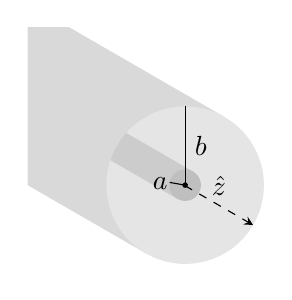
\begin{tikzpicture}[]
\clip (-2,-1.1) rectangle (1,2);
\begin{scope}[rotate=-30]
\fill[gray!30] (-3,-1) rectangle (0,1);
\fill[gray!20] (0,0) circle(1cm);
\begin{scope}
\clip(0,0) circle(1cm);
\fill[gray!40] (-3,-0.2) rectangle (0,0.2);
\fill[gray!50] (0,0) circle(2mm);
\fill[black] (0,0) circle (1pt); % origin
\end{scope}
\draw (120:0) -- node[right]{$b$}(120:1);
\draw (200:0) -- node[left]{$a$}(200:0.2);
\draw[-stealth, dashed] ([yshift=-0.5\pgflinewidth]0,0) -- node[above]{$\hat{z}$}([yshift=-0.5\pgflinewidth]1,0);
\end{scope}

\end{tikzpicture}%
} % end scalebox

\begin{tikzpicture}
\draw[pattern=north west lines, pattern color=gray!50!white] (0,0) circle (1.5);
\draw[black,fill=white] (0,0) circle (0.5);
\fill[black] (0,0) circle (1pt); % origin
\draw (120:0.5) -- node[right]{$b$}(120:1.5);
\draw (200:0) -- node[above]{$a$}(200:0.5);
\draw[dashed, -stealth] (90:0) -- (90:2);
 \draw[-stealth] (0,1.75) arc (90:120:1.5) node[above]{$\phi$};
\end{tikzpicture}
\end{textblock}

\begin{textblock}{7}(7,2.5)
	
	\visible<0|handout:1>{
	\alert{
	\begin{small}
	\eq{
			&\oiint_S \vec{E}\mycdot\vec{dS} = \dfrac{Q_{\text{enclosed}}}{\varepsilon} \\
			&\vec{E} = \rhohat E_{\rho} + \phihat E_{\phi} + \zhat E_z \\
			&\vec{dS} = \rhohat \rho dz d\phi \\
			&\implies \int_{0}^{2\pi} \int_{0}^{L} E_{\rho} \rho dz d\phi =  \dfrac{Q_{\text{enclosed}}}{\varepsilon} \\
			&\implies E_{\rho} \rho 2\pi L = \dfrac{1}{\varepsilon} \iiint \rho_V dV \\
			&\implies \rho_V = \dfrac{Q_{\text{tot}}}{\text{volume}} = \dfrac{Q_{\text{tot}}}{ \pi a^2 L} \\
			&\implies E_{\rho} \rho 2\pi L = \dfrac{1}{\varepsilon} \iiint \dfrac{Q_{\text{tot}}}{ \pi a^2 L} dV \\
			&\implies E_{\rho} \rho 2\pi L = \dfrac{Q_{\text{tot}}}{ \pi a^2 L \varepsilon} \int_{0}^{\rho_0} \rho d\rho \int_{0}^{2\pi} d\phi \int_{0}^{L} dz \\
	} % end eq
	\end{small}
	} %end alert
	} % end visible

	
\end{textblock}

\end{frame}

% coaxial cable
%%%%%%%%%%%%%%%%%%%%%%%%%%%%%%%%%%%%%%%%%%%%%%%%%%%%%%
%%%%%%%%%%%%%%%%%%%%%%%%%%%%%%%%%%%%%%%%%%%%%%%%%%%%%%

\begin{frame}{Gauss' Law: Coaxial Cable (cont'd)}

\begin{textblock}{14.5}(0.5,3)
\scalebox{1.25}{
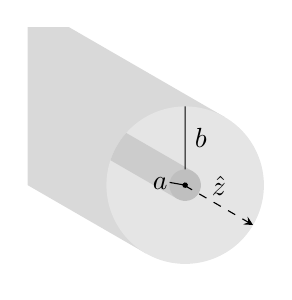
\begin{tikzpicture}[]
\clip (-2,-1.1) rectangle (1,2);
\begin{scope}[rotate=-30]
\fill[gray!30] (-3,-1) rectangle (0,1);
\fill[gray!20] (0,0) circle(1cm);
\begin{scope}
\clip(0,0) circle(1cm);
\fill[gray!40] (-3,-0.2) rectangle (0,0.2);
\fill[gray!50] (0,0) circle(2mm);
\fill[black] (0,0) circle (1pt); % origin
\end{scope}
\draw (120:0.2) -- node[right]{$b$}(120:1);
\draw (200:0) -- node[left]{$a$}(200:0.2);
\draw[-stealth, dashed] ([yshift=-0.5\pgflinewidth]0,0) -- node[above]{$\hat{z}$}([yshift=-0.5\pgflinewidth]1,0);
\end{scope}

\end{tikzpicture}%
} % end scalebox

\begin{tikzpicture}
\draw[pattern=north west lines, pattern color=gray!50!white] (0,0) circle (1.5);
\draw[black,fill=white] (0,0) circle (0.5);
\fill[black] (0,0) circle (1pt); % origin
\draw (120:0.5) -- node[right]{$b$}(120:1.5);
\draw (200:0) -- node[above]{$a$}(200:0.5);
\draw[dashed, -stealth] (90:0) -- (90:2);
 \draw[-stealth] (0,1.75) arc (90:120:1.5) node[above]{$\phi$};
\end{tikzpicture}
\end{textblock}

\begin{textblock}{7}(8,2.5)
	
	\visible<0|handout:1>{
	\alert{
	\begin{small}
	\eq{
			&\oiint_S \vec{E}\mycdot\vec{dS} = \dfrac{Q_{\text{enclosed}}}{\varepsilon} \\
			 &E_{\rho} \rho 2\pi L = \dfrac{Q_{\text{tot}}}{ \pi a^2 L \varepsilon} \lp \rho^2_0 \rp \lp 2\pi  \rp\lp L \rp \\
			 &E_{\rho} = \dfrac{Q_{\text{tot}} \rho^2_0}{2\pi\varepsilon a^2 L \rho} 
	} % end eq
	\end{small}
	} %end alert
	} % end visible

	
\end{textblock}

\end{frame}


% coaxial cable
%%%%%%%%%%%%%%%%%%%%%%%%%%%%%%%%%%%%%%%%%%%%%%%%%%%%%%
%%%%%%%%%%%%%%%%%%%%%%%%%%%%%%%%%%%%%%%%%%%%%%%%%%%%%%

\begin{frame}{Gauss' Law: Coaxial Cable (cont'd)}

\begin{textblock}{14.5}(0.5,3)
\scalebox{1.25}{
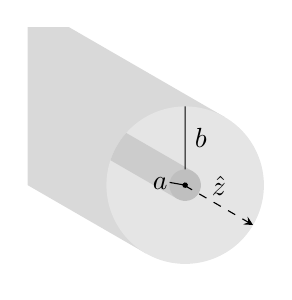
\begin{tikzpicture}[]
\clip (-2,-1.1) rectangle (1,2);
\begin{scope}[rotate=-30]
\fill[gray!30] (-3,-1) rectangle (0,1);
\fill[gray!20] (0,0) circle(1cm);
\begin{scope}
\clip(0,0) circle(1cm);
\fill[gray!40] (-3,-0.2) rectangle (0,0.2);
\fill[gray!50] (0,0) circle(2mm);
\fill[black] (0,0) circle (1pt); % origin
\end{scope}
\draw (120:0.2) -- node[right]{$b$}(120:1);
\draw (200:0) -- node[left]{$a$}(200:0.2);
\draw[-stealth, dashed] ([yshift=-0.5\pgflinewidth]0,0) -- node[above]{$\hat{z}$}([yshift=-0.5\pgflinewidth]1,0);
\end{scope}

\end{tikzpicture}%
} % end scalebox

\begin{tikzpicture}
\draw[pattern=north west lines, pattern color=gray!50!white] (0,0) circle (1.5);
\draw[black,fill=white] (0,0) circle (0.5);
\fill[black] (0,0) circle (1pt); % origin
\draw (120:0.5) -- node[right]{$b$}(120:1.5);
\draw (200:0) -- node[above]{$a$}(200:0.5);
\draw[dashed, -stealth] (90:0) -- (90:2);
 \draw[-stealth] (0,1.75) arc (90:120:1.5) node[above]{$\phi$};
\end{tikzpicture}
\end{textblock}

\begin{textblock}{7}(8,2.5)
	
%	\visible<0|handout:1>{
%	\alert{
%	\begin{small}
%	\eq{
%			&\text{Case 1: } 
%			 &E_{\rho} = \dfrac{Q_{\text{tot}} \rho^2_0}{2\pi\varepsilon a^2 L \rho} 
%	} % end eq
%	\end{small}
%	} %end alert
%	} % end visible

	
\end{textblock}

\end{frame}

\end{lesson22}
%%%%%%%%%%%%%%%%%%%%%%%%%%%%%%%%%%%%%%%%%%%%%%%%%%%%%%%%%%%%%%
%%%%%%%%%%%%%%%%%%%%%%%%%%%%%%%%%%%%%%%%%%%%%%%%%%%%%%%%%%%%%%
\begin{lesson23}

\begin{frame}{Scalar Potential: Line Charge}
\begin{textblock}{7}(0.5,4)
\begin{tikzpicture}[scale=0.7]
		\def\qonex{0}
		\def\qoney{3}
		\def\qtwox{0}
		\def\qtwoy{-2}
		\def\qthreex{4}
		\def\qthreey{0}
		\begin{axis}[ 
		domain=-5:5,
%		samples=200, 
%		xmin=-1, 
		xmax=2.5, 
		ymax=3.5,
		ymin=-3.5,
%		title={Single Square Pulse, $\Pi (\frac{t}{\tau})$},
%		scaled x ticks=base 10:6,
%		xtick scale label code/.code={},
%		minor x tick num = 5,
%		minor y tick num = 5,
		ytick={-3,3},
		yticklabels={-a,a},
		xtick=\empty,
%		xticklabels={$\rho$},
		xlabel={$\rho$},
		ylabel={$z$},
		axis y line = middle,
		axis x line = middle,
		x label style={xshift=0.5cm},
		x label style={yshift=-0.25cm},
		y label style ={xshift=-0.75cm},
		y label style = {yshift =0.5cm},
		yticklabel shift=0.5cm,
		clip=false,
		]
%		\node[cylinder, shape border rotate=90, draw, minimum height=6.5cm, minimum width=0.5cm] at (0,0) {};
		\addplot[ultra thick, red] coordinates {(0,-3)(0,3)};
		\node[red] at (-0.5,0) {$\rho_\ell$};
		\addplot[blue, dashed, ->] (0,1.5) -- (1.5,0) node[midway, above, blue]{r};
		
		\end{axis}
\end{tikzpicture}
\end{textblock}
\begin{textblock}{7}(8,2.25)

	\visible<0|handout:1>{
	\alert{
	\begin{small}
	\eq{
        	&V = \int \dfrac{dQ}{4\pi\varepsilon r} \\
        	&dQ = \rho_\ell d\ell = \rho_\ell dz \\
        	& r = \sqrt{z^2 + \rho^2} \\
        	&\implies  \int \dfrac{\rho_\ell dz}{4\pi\varepsilon \sqrt{z^2 + \rho^2} } \\
        	&= \dfrac{\rho_\ell}{4\pi \varepsilon} \int \dfrac{1}{\sqrt{z^2 + \rho^2}} dz \\
        	&=\dfrac{2\rho_\ell}{4\pi \varepsilon} \lb \text{ln} \lp z + \sqrt{z^2 + \rho^2} \rp \rb\Bigg|_0^a \\
        	&V=\dfrac{\rho_\ell}{2\pi\varepsilon}\lb \text{ln} \lp \dfrac{a + \sqrt{a^2 + \rho^2}}{\rho} \rp \rb
	} % end eq
	\end{small}
	} %end alert
	} % end visible
	
	
\end{textblock}
\end{frame}

%%%%%%%%%%%%%%%%%%%%%%%%%%%%%%%%%%%%%%%%%%%%%%%%%%%%%%
%%%%%%%%%%%%%%%%%%%%%%%%%%%%%%%%%%%%%%%%%%%%%%%%%%%%%%

\begin{frame}{Scalar Potential: Line Charge}
\begin{textblock}{7}(0.5,4)
\begin{tikzpicture}[scale=0.7]
		\def\qonex{0}
		\def\qoney{3}
		\def\qtwox{0}
		\def\qtwoy{-2}
		\def\qthreex{4}
		\def\qthreey{0}
		\begin{axis}[ 
		domain=-5:5,
%		samples=200, 
%		xmin=-1, 
		xmax=2.5, 
		ymax=3.5,
		ymin=-3.5,
%		title={Single Square Pulse, $\Pi (\frac{t}{\tau})$},
%		scaled x ticks=base 10:6,
%		xtick scale label code/.code={},
%		minor x tick num = 5,
%		minor y tick num = 5,
		ytick={-3,3},
		yticklabels={-a,a},
		xtick=\empty,
%		xticklabels={$\rho$},
		xlabel={$\rho$},
		ylabel={$z$},
		axis y line = middle,
		axis x line = middle,
		x label style={xshift=0.5cm},
		x label style={yshift=-0.25cm},
		y label style ={xshift=-0.75cm},
		y label style = {yshift =0.5cm},
		yticklabel shift=0.5cm,
		clip=false,
		]
%		\node[cylinder, shape border rotate=90, draw, minimum height=6.5cm, minimum width=0.5cm] at (0,0) {};
		\addplot[ultra thick, red] coordinates {(0,-3)(0,3)};
		\node[red] at (-0.5,0) {$\rho_L$};
		\addplot[blue, dashed, ->] (0,1.5) -- (1.5,0) node[midway, above, blue]{r};
		
		\end{axis}
\end{tikzpicture}
\end{textblock}
\begin{textblock}{7}(8.5,2.75)

	\visible<0|handout:1>{
	\alert{
	\begin{small}
	\eq{
        	&V=\dfrac{\rho_\ell}{2\pi\varepsilon}\lb \text{ln} \lp \dfrac{a + \sqrt{a^2 + \rho^2}}{\rho} \rp \rb \\
        	&\implies\vec{E} = -\nabla V = -\rhohat \partd{V}{\rho} \\
        	&\text{for } a >> \rho \text{ :} \\
        	&\implies \vec{E} = -\rhohat \partd{}{\rho}\dfrac{\rho_\ell}{2\pi\varepsilon}\lb \text{ln} \lp \dfrac{2a }{\rho} \rp \rb \\
        	& = -\rhohat \partd{}{\rho}\dfrac{\rho_\ell}{2\pi\varepsilon}\lb \text{ln} \lp 2a \rp - \text{ln}\lp \rho\rp \rb \\
        	&\implies \vec{E} = \rhohat \dfrac{\rho_L}{2\pi \varepsilon \rho}     	
	} % end eq
	\end{small}
	} %end alert
	} % end visible
	
\end{textblock}
\end{frame}

%%%%%%%%%%%%%%%%%%%%%%%%%%%%%%%%%%%%%%%%%%%%%%%%%%%%%%
%%%%%%%%%%%%%%%%%%%%%%%%%%%%%%%%%%%%%%%%%%%%%%%%%%%%%%

\begin{frame}{1D Boundary Value Problem}

\begin{textblock}{6}(0.5,3)
\begin{center}
\begin{circuitikz}[scale=1]
	\draw (0,0) to[battery,a_=\myv{0}] ++(0,3)
					to[short] ++(3,0)
					to[short] ++(0,-0.75)
					to[open] ++(0,-1.5)
					to[short] ++(0,-0.75)
					to[short] ++(-3,0);
	\node[ground] at (1.5,0){};
	% draw the capacitor
	\fill[pattern=north west lines, pattern color=gray!50!white] (1.25,0.75) rectangle (4.75,2.25);
	\draw[thick] (1.25,2.25) -- (4.75,2.25) node[right] {$z=d$}; % top wall
	\draw[thick] (1.25,0.75) -- (4.75,0.75) node[right] {$z=0$}; % bottom
	\foreach \x in {2,2.15,...,4}
	{
		\node at (\x,2.5){\tiny +};
		\node at (\x,0.5){\tiny -};
	}
\end{circuitikz}
\end{center}

\alert{
\eq{
	V &= \dfrac{\myv{s}}{d} z \\
	\vec{E} &=  -\nabla V = -\zhat\partd{}{z} \lp \dfrac{\myv{s}}{d} z \rp = -\zhat\dfrac{\myv{s}}{d}
} % end eq
} % end alert

\end{textblock}

\end{frame}

%%%%%%%%%%%%%%%%%%%%%%%%%%%%%%%%%%%%%%%%%%%%%%%%%%%%%%
%%%%%%%%%%%%%%%%%%%%%%%%%%%%%%%%%%%%%%%%%%%%%%%%%%%%%%

\begin{frame}{Gauss' Law: Point (differential) Form}
\begin{textblock}{14.5}(0.5,3)

	\begin{myblock}[0.9]{Derivation}
		\eq{
			&\oiint \vec{D} \mycdot \vec{dS} = Q_{\text{encl}} \\
			&\iiint_V \nabla\mycdot \vec{D} dV = \iiint_V \rho_V dV  \\
			&\nabla \mycdot \vec{D} = \rho_V \\
			&\nabla \mycdot \vec{E} = \dfrac{\rho_V}{\varepsilon} \\
		}
	\vspace{-0.5in}

\end{myblock}

\end{textblock}
\end{frame}
%%%%%%%%%%%%%%%%%%%%%%%%%%%%%%%%%%%%%%%%%%%%%%%%%%%%%%
%%%%%%%%%%%%%%%%%%%%%%%%%%%%%%%%%%%%%%%%%%%%%%%%%%%%%%

\begin{frame}{Example}
\begin{textblock}{14.5}(0.5,3)
Given the following static electric field in free space, find the charge density ($\rho$) at the point $(2,-2,0)$

\vspace{-16pt}

\eq{
	&\vec{E} (\vec{r} ) = \xhat A x^2 + \yhat B z + \zhat C x^2 z \longrightarrow  A = 3 \volts/\text{m}^3 \quad B = 2 \volts/\text{m}^3\quad C = 1 \volts/\text{m}^4
}

	\vspace{-18pt}
	\begin{myblock}[0.9]{Solution}
	\vspace{-12pt}
	\begin{small}
		\alert{
		\eq{
			\nabla\mycdot\vec{E} &= \dfrac{\rho}{\varepsilon_0} \\
			\varepsilon_0 \lb \partd{}{x} \lp 3x^2 \rp + \partd{}{y} \lp 2z \rp + \partd{}{z}\lp x^2 z \rp \rb &= \rho \\
			\varepsilon_0 \lp 6x + 0 + x^2 \rp &= \rho \\
			8.854\ee{-12}\text{F/m} \lb (6)(2) + 2^2 \rb &= \rho \\
			141.7 \text{pC/m}^3 = \rho
		}
		\vspace{-12pt}
		}
	\end{small}
	\end{myblock}

\end{textblock}
\end{frame}

%%%%%%%%%%%%%%%%%%%%%%%%%%%%%%%%%%%%%%%%%%%%%%%%%%%%%%%%%%%%%%%
%%%%%%%%%%%%%%%%%%%%%%%%%%%%%%%%%%%%%%%%%%%%%%%%%%%%%%%%%%%%%%%

\section{Electric Field Boundary Conditions}
\begin{frame}{Static Electric Fields with Boundary}
\begin{textblock}{14.5}(0.5,4)
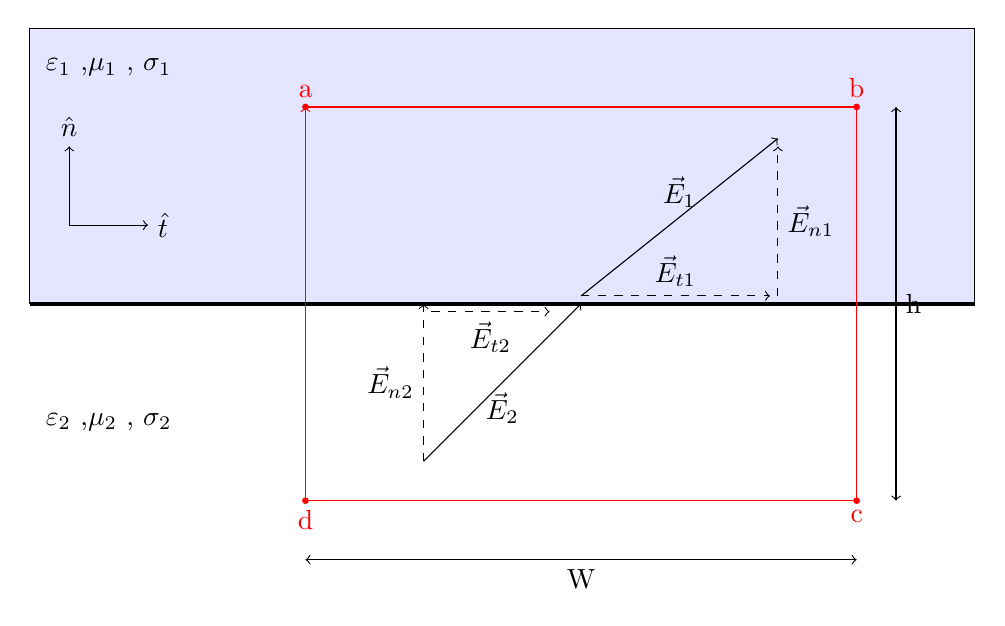
\begin{tikzpicture}

	\draw[fill=blue!10!white] (0,0) rectangle (12,3.5);
	\draw[ultra thick, black] (0,0) --++ (12,0);
	\node at (1,3) {$\varepsilon_1$ ,$\mu_1$ , $\sigma_1 $};
	\node at (1,-1.5) {$\varepsilon_2$ ,$\mu_2$ , $\sigma_2 $};
	
	\draw[->] (0.5,1) --++ (1,0) node[right] {$\hat{t}$};
	\draw[->] (0.5,1) --++ (0,1) node[above] {$\hat{n}$};
	
	% material 2
	\draw[->] (5,-2) --++ (2,2) node[midway, below] {$\vec{E}_2$}; 
	\draw[->, dashed] (5,-2) --++ (0,2) node[left, midway] {$\vec{E}_{\text{n2}}$};
	\draw[->, dashed] (5.1,-0.1) --++ (1.5,0) node[below, midway] {$\vec{E}_{\text{t2}}$};
	
	% material 1
	\draw[->] (7, 0.1)  --++ (2.5,2) node[midway, above] {$\vec{E}_{1}$};
	\draw[->, dashed] (9.5, 0.1) --++ (0,1.9) node[right, midway] {$\vec{E}_{\text{n1}}$};
	\draw[->, dashed] (7,0.1) --++ (2.4,0) node[above, midway] {$\vec{E}_{\text{t1}}$};
	
	%contours
	\coordinate (a) at (3.5, 2.5);
	\coordinate (b) at (10.5, 2.5);
	\coordinate (c) at (10.5, -2.5);
	\coordinate (d) at (3.5, -2.5);	
	
	\draw[red, fill=red] (a) circle (1pt) node[above]  {a};
	\draw[red, fill=red] (b) circle (1pt) node[above]  {b};
	\draw[red, fill=red] (c) circle (1pt) node[below] {c};
	\draw[red, fill=red] (d) circle (1pt) node[below] {d};
	
	\path[draw=red, ->] (a) -| (b) -| (c) -| (d) -| (a);
	\draw[<->] (3.5,-3.25) --++ (7,0) node[midway, below] {W};
	\draw[<->] (11,2.5) --++(0,-5) node[midway, right] {h};
	%\draw[red, thick,->] (3.5,2.5) node[above left] {a} --++ (7,0) node[above right] {b} --++ (0,-5) node[below right] {c} --++ (-7,0) node[below left] {d} --++ (0,5);
\end{tikzpicture}

\end{textblock}
\end{frame}


%%%%%%%%%%%%%%%%%%%%%%%%%%%%%%%%%%%%%%%%%%%%%%%%%%%%%%%%%%%%%%%
%%%%%%%%%%%%%%%%%%%%%%%%%%%%%%%%%%%%%%%%%%%%%%%%%%%%%%%%%%%%%%%
\begin{frame}{Boundary Conditions: Transverse}
\begin{textblock}{14.5}(0.5,2)
\alert{
\eq{
	&\oint \myvec{E}\mycdot \vec{d\ell} = 0 \\ 
	&\int\myvec{E}\mycdot \vec{d\ell_{ab}} +  	\int\myvec{E}\mycdot \vec{d\ell_{bc}} + 	\int\myvec{E}\mycdot \vec{d\ell_{cd}} + 	\int\myvec{E}\mycdot \vec{d\ell_{da}} = 0 \\
	&\int\myvec{E}\mycdot \vec{d\ell_{ab}} = \int_a^b \myvec{E}_{\text{t1}}\mycdot \hat{t} d\ell = E_{\text{t1}} W\\
	&\int\myvec{E}\mycdot \vec{d\ell_{bc}} = \int_{b-h/2}^b \myvec{E}_{1}\mycdot \lp-\hat{n} \rp d\ell + 
	\int_{b-h/2}^c \myvec{E}_{2}\mycdot \lp-\hat{n} \rp d\ell =-\lp E_{\text{n1}} + E_{\text{n2}} \rp\dfrac{h}{2}  \\
	&\int\myvec{E}\mycdot \vec{d\ell_{cd}} = \int_c^d \myvec{E}_{\text{t2}}\mycdot \lp -\hat{t}\rp d\ell = -E_{\text{t2}} W\\
	&\int\myvec{E}\mycdot \vec{d\ell_{da}} = \int_d^{d+h/2} \myvec{E}_{2}\mycdot \lp \hat{n} \rp d\ell +
	\int_{d+h/2}^a \myvec{E}_{1}\mycdot \lp \hat{n} \rp d\ell = \lp E_{\text{n1}} + E_{\text{n2}} \rp\dfrac{h}{2}  \\
	&\implies \oint \myvec{E}\mycdot \vec{d\ell} =  E_{\text{t1}} W + -\lp E_{\text{n1}} + E_{\text{n2}} \rp\dfrac{h}{2} -E_{\text{t2}} W +  \lp E_{\text{n1}} + E_{\text{n2}} \rp\dfrac{h}{2} = 0 
} % end eq
}% end alert
\end{textblock}
\end{frame}

%%%%%%%%%%%%%%%%%%%%%%%%%%%%%%%%%%%%%%%%%%%%%%%%%%%%%%%%%%%%%%%
%%%%%%%%%%%%%%%%%%%%%%%%%%%%%%%%%%%%%%%%%%%%%%%%%%%%%%%%%%%%%%%
\begin{frame}{Boundary Conditions: Transverse}
\begin{textblock}{14.5}(0.5,4)
\begin{myblock}[0.9]{Transverse}
\alert{
\eq{
	E_{\text{t1}} = E_{\text{t2}} \qquad \text{ or } \qquad \hat{n}_{21} \times \lp \vec{E}_{1} - \vec{E}_2 \rp = 0 
} % end eq
}% end alert
\end{myblock}
\end{textblock}
\end{frame}
\end{lesson23} 
%%%%%%%%%%%%%%%%%%%%%%%%%%%%%%%%%%%%%%%%%%%%%%%%%%%%%%%%%%%%%%%
%%%%%%%%%%%%%%%%%%%%%%%%%%%%%%%%%%%%%%%%%%%%%%%%%%%%%%%%%%%%%%%
\begin{lesson24}
\begin{frame}{Boundary Conditions: Normal}
\begin{textblock}{14.5}(0.5,3.5)
\begin{tikzpicture}

	\draw[fill=blue!10!white] (0,0) rectangle (12,3.5);
	\draw[ultra thick, black] (0,0) --++ (12,0);
	\node at (1,3) {$\varepsilon_1$ ,$\mu_1$ , $\sigma_1 $};
	\node at (1,-1.5) {$\varepsilon_2$ ,$\mu_2$ , $\sigma_2 $};
	
	\draw[->] (0.5,1) --++ (1,0) node[right] {$\hat{t}$};
	\draw[->] (0.5,1) --++ (0,1) node[above] {$\hat{n}$};
	
	% material 2
	\draw[->] (5,-2) --++ (2,2) node[midway, below] {$\vec{E}_2$}; 
	\draw[->, dashed] (5,-2) --++ (0,2) node[left, midway] {$\vec{E}_{\text{n2}}$};
	\draw[->, dashed] (5.1,-0.1) --++ (1.5,0) node[below, midway] {$\vec{E}_{\text{t2}}$};
	
	% material 1
	\draw[->] (7, 0.1)  --++ (2.5,2) node[midway, above] {$\vec{E}_{1}$};
	\draw[->, dashed] (9.5, 0.1) --++ (0,1.9) node[right, midway] {$\vec{E}_{\text{n1}}$};
	\draw[->, dashed] (7,0.1) --++ (2.4,0) node[above, midway] {$\vec{E}_{\text{t1}}$};
	\foreach\x in {0.5,1,1.5,...,11}{
		\node[red] at (\x,0.1) {+};
	}	
	
	\node[cylinder, shape border rotate=90, draw, minimum height=5cm, minimum width=7cm, red] at (7,0) {};
	
\end{tikzpicture}

\vspace{-16pt}
\alert{
\eq{
	\implies \oiint \vec{D} \mycdot \vec{dS} &= \rho_S
} % end eq
} % end alert
\end{textblock}
\end{frame}

%%%%%%%%%%%%%%%%%%%%%%%%%%%%%%%%%%%%%%%%%%%%%%%%%%%%%%%%%%%%%%%
%%%%%%%%%%%%%%%%%%%%%%%%%%%%%%%%%%%%%%%%%%%%%%%%%%%%%%%%%%%%%%%
\begin{frame}{Boundary Conditions: Normal}
\begin{textblock}{14.5}(0.5,3)
\alert{
\eq{
	&\text{Top } \longrightarrow \oiint \vec{D}\mycdot \vec{dS}_{\text{top}} = \oiint \vec{D}\mycdot \hat{n} dS = D_{\text{n1}} (\text{area}) \\
	&\text{Bottom } \longrightarrow \oiint \vec{D}\mycdot \vec{dS}_{\text{bottom}} = \oiint \vec{D}\mycdot \lp -\hat{n}\rp dS = -D_{\text{n2}} (\text{area}) \\
	&\text{Sides } \overset{h\rightarrow 0}{\longrightarrow} \oiint\vec{D}\mycdot\vec{dS}_{\text{sides}} = 0 
	&Q_{\text{enclosed}} \longrightarrow \iint \rho_S dS = \rho_S (\text{area}) \\
	&\implies D_{\text{n1}} - D_{\text{n2}} = \rho_S \qquad \text{or} \qquad \hat{n}_{21} \mycdot \lp \varepsilon_1 \vec{E}_1 - \varepsilon_2 \vec{E}_2 \rp = \rho_S
} % end eq
} % end alert
\end{textblock}
\end{frame}


%%%%%%%%%%%%%%%%%%%%%%%%%%%%%%%%%%%%%%%%%%%%%%%%%%%%%%%%%%%%%%%
%%%%%%%%%%%%%%%%%%%%%%%%%%%%%%%%%%%%%%%%%%%%%%%%%%%%%%%%%%%%%%%
\begin{frame}{Boundary Conditions: Summary}
\begin{textblock}{14.5}(0.5,4)
\begin{myblock}[0.9]{Electric Field Boundary Conditions}
\eq{
&\text{ Transverse: } \qquad \hat{n}_{21} \times \lp \vec{E}_1 - \vec{E}_2 \rp = 0 \\
&\text{ Normal: } \qquad \hat{n}_{21} \mycdot \lp \varepsilon_1 \vec{E}_1 - \varepsilon_2 \vec{E}_2 \rp = \rho_S
} % end eq
\end{myblock}
\end{textblock}
\end{frame}

%%%%%%%%%%%%%%%%%%%%%%%%%%%%%%%%%%%%%%%%%%%%
%%%%%%%%%%%%%%%%%%%%%%%%%%%%%%%%%%%%%%%%%%%%

\begin{frame}{Angle of Incidence}
\begin{textblock}{14.5}(0.5,4)
\begin{tikzpicture}

	\draw[fill=blue!10!white] (0,0) rectangle (12,3.5);
	\draw[ultra thick, black] (0,0) --++ (12,0);
	\node at (1,3) {$\varepsilon_1$ ,$\mu_1$ , $\sigma_1 $};
	\node at (1,-1.5) {$\varepsilon_2$ ,$\mu_2$ , $\sigma_2 $};
	
	\draw[->] (0.5,1) --++ (1,0) node[right] {$\hat{t}$};
	\draw[->] (0.5,1) --++ (0,1) node[above] {$\hat{n}$};
	
	% material 2
	\draw[->] (5,-2) --++ (2,2) node[midway, below] {$\vec{E}_2$}; 
	\draw[->, dashed] (5,-2) --++ (0,2) node[left, midway] {$\vec{E}_{\text{n2}}$};
	\draw[->, dashed] (5.1,-0.1) --++ (1.5,0) node[above, midway] {$\vec{E}_{\text{t2}}$};
	
	% material 1
	\draw[->] (7, 0.1)  --++ (2.5,2) node[midway, above] {$\vec{E}_{1}$};
	\draw[->, dashed] (9.5, 0.1) --++ (0,1.9) node[right, midway] {$\vec{E}_{\text{n1}}$};
	\draw[->, dashed] (7,0.1) --++ (2.4,0) node[below, midway] {$\vec{E}_{\text{t1}}$};
	
	% plane of incidence
	\draw[dashed, ultra thick, blue] (7,-2.5) --++ (0,5) node[above, blue] {Plane of Incidence}; 
	\draw[<-, red] (7.5,0.5) arc (45:110:0.5) node[midway, above] {$\theta_1$};
	\draw[<-, red] (6.5,-0.5) arc (225:290:0.5) node[midway, below] {$\theta_2$};
	\node[red, align=left] at (10,-2) {$\theta_1 = \text{tan}^{-1}\lp \dfrac{|E_{t1}|}{|E_{n1}|} \rp$ \\ $\theta_2 = \text{tan}^{-1}\lp \dfrac{|E_{t2}|}{|E_{n2}|} \rp$};
\end{tikzpicture}

\end{textblock}
\end{frame}

%%%%%%%%%%%%%%%%%%%%%%%%%%%%%%%%%%%%%%%%%%%%%%%%%%%%%%%%%%%%%%%
%%%%%%%%%%%%%%%%%%%%%%%%%%%%%%%%%%%%%%%%%%%%%%%%%%%%%%%%%%%%%%%
\begin{frame}{Boundary Conditions: Example}
\begin{textblock}{14.5}(0.5,3.5)
An electric field $\vec{E}_1$ is incident from free space onto a material with $\varepsilon_{2r} = 2$. If  $\vec{E}_2 = \xhat 3 + \yhat 4 + \zhat 5$, find $\vec{E}_1$ and the angle of incidence of each vector.

\vspace{12pt}

\scalebox{0.65}{
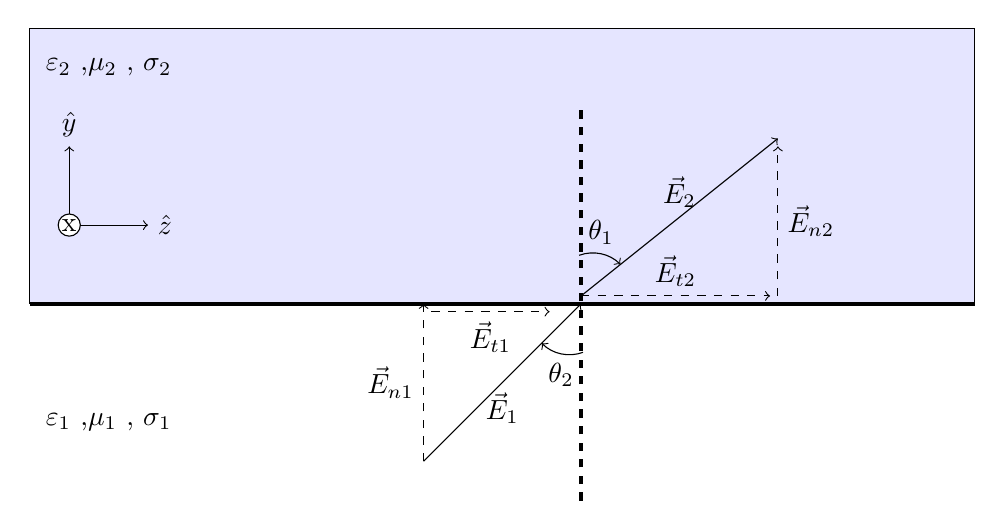
\begin{tikzpicture}

	\draw[fill=blue!10!white] (0,0) rectangle (12,3.5);
	\draw[ultra thick, black] (0,0) --++ (12,0);
	\node at (1,3) {$\varepsilon_2$ ,$\mu_2$ , $\sigma_2 $};
	\node at (1,-1.5) {$\varepsilon_1$ ,$\mu_1$ , $\sigma_1 $};
	
	\draw[->] (0.5,1) --++ (1,0) node[right] {$\hat{z}$};
	\draw[->] (0.5,1) --++ (0,1) node[above] {$\hat{y}$};
	\draw[black, fill=white] (0.5,1) circle (4pt) node {x};
	
	% material 1
	\draw[->] (5,-2) --++ (2,2) node[midway, below] {$\vec{E}_1$}; 
	\draw[->, dashed] (5,-2) --++ (0,2) node[left, midway] {$\vec{E}_{\text{n1}}$};
	\draw[->, dashed] (5.1,-0.1) --++ (1.5,0) node[below, midway] {$\vec{E}_{\text{t1}}$};
	
	% material 2
	\draw[->] (7, 0.1)  --++ (2.5,2) node[midway, above] {$\vec{E}_{2}$};
	\draw[->, dashed] (9.5, 0.1) --++ (0,1.9) node[right, midway] {$\vec{E}_{\text{n2}}$};
	\draw[->, dashed] (7,0.1) --++ (2.4,0) node[above, midway] {$\vec{E}_{\text{t2}}$};
	
	
	
	% plane of incidence
	\draw[dashed, ultra thick] (7,-2.5) --++ (0,5); 
	\draw[<-] (7.5,0.5) arc (45:110:0.5) node[midway, above] {$\theta_1$};
	\draw[<-] (6.5,-0.5) arc (225:290:0.5) node[midway, below] {$\theta_2$};
	
\end{tikzpicture}
} % end scalebox
\end{textblock}
\begin{textblock}{5}(10,6)
\alert{
\begin{small}
\eq{
	&\text{Transverse} \longrightarrow  \xhat, \zhat\\
	&\text{Normal} \longrightarrow \yhat \\
	} % end eq
\end{small}
	} % end alert
\end{textblock}
\end{frame}

%%%%%%%%%%%%%%%%%%%%%%%%%%%%%%%%%%%%%%%%%%%%%%%%%%%%%%%%%%%%%%%
%%%%%%%%%%%%%%%%%%%%%%%%%%%%%%%%%%%%%%%%%%%%%%%%%%%%%%%%%%%%%%%
\begin{frame}{Boundary Conditions: Example (cont'd)}
\begin{textblock}{8.5}(0.5,3)
\alert{
\begin{small}
\eq{
	&\circled{1} 
	\begin{cases}
		&\vec{E}_{\text{t2}} = \xhat 3 + \zhat 5 \implies | \vec{E}_{\text{t2}} | = \sqrt{3^2 + 5^2} = \sqrt{34}  \\
		&\vec{E}_{\text{n2}} = \yhat 4 \implies |\vec{E}_{\text{n2}}| = 4
	\end{cases} \\
	&\circled{2} \longrightarrow \theta_2 = \text{tan}^{-1} \lp \dfrac{| \vec{E}_{\text{t2}} | }{| \vec{E}_{\text{n2}} | } \rp =  \text{tan}^{-1} \lp \dfrac{\sqrt{34} }{4 } \rp = 55.6\mydeg \\
	&\circled{3} \longrightarrow \text{Normal BC}  \implies \hat{n}_{2,1} = -\yhat \\
	&\qquad -\yhat \mycdot \lp \varepsilon_1 \vec{E}_1 - \varepsilon_2 \vec{E}_2 \rp = 0  \\
	&\qquad -\yhat \mycdot \varepsilon_0 \vec{E}_1 + \yhat \mycdot \lb 2\varepsilon_0 \lp \xhat 3 + \yhat 4 + \zhat 5 \rp\rb = 0 \\
	&\qquad -\varepsilon_0 E_{1y} + 8\varepsilon_0 = 0 \\
	&\qquad \implies E_{1y}  = 8
} % end eq
\end{small}
} % end alert
\end{textblock}
\end{frame}

%%%%%%%%%%%%%%%%%%%%%%%%%%%%%%%%%%%%%%%%%%%%%%%%%%%%%%%%%%%%%%%
%%%%%%%%%%%%%%%%%%%%%%%%%%%%%%%%%%%%%%%%%%%%%%%%%%%%%%%%%%%%%%%
\begin{frame}{Boundary Conditions: Example (cont'd)}
\begin{textblock}{8.5}(0.5,3)
\alert{
\begin{small}
\eq{
	&\circled{4} \longrightarrow \text{Transverse BC}  \\
%	&\qquad \implies \vec{E}_{\text{t1}} = \vec{E}_{\text{t2}} \implies \vec{E}_{\text{t1} = \xhat 3 + \zhat 5 \\
	&\circled{5} \longrightarrow \vec{E}_1 = \xhat 3 + \yhat 8 + \zhat 5 \\
	&\circled{6} \longrightarrow \theta_1 = \text{tan}^{-1}\lp\dfrac{|\vec{E}_{\text{t1}}|}{|\vec{E}_{\text{n1}}|}\rp = \text{tan}^{-1}\lp \dfrac{\sqrt{34}}{8}\rp = 36\mydeg
} % end eq
\end{small}
} % end alert
\end{textblock}

\begin{textblock}{14.5}(0.5,8)
\begin{myblock}[0.9]{Summary}
\vspace{-12pt}
\alert{
\eq{
	\vec{E}_1 &= \xhat 3 + \yhat 8 + \zhat 5  \\
	\vec{E}_2 &= \xhat 3 + \yhat 4 + \zhat 5  \\
	\theta_1 &= 36\mydeg \\
	\theta_2 &= 55.6\mydeg
} % end eq
}% end alert
\vspace{-12pt}
\end{myblock}
\end{textblock}
\end{frame}
%%%%%%%%%%%%%%%%%%%%%%%%%%%%%%%%%%%%%%%%%%%%%%%%%%%%%%%%%%%%%%%
%%%%%%%%%%%%%%%%%%%%%%%%%%%%%%%%%%%%%%%%%%%%%%%%%%%%%%%%%%%%%%%
\begin{frame}{Your Turn: Example \#2}
\begin{textblock}{14.5}(0.5,3.5)
An electric field $\vec{E}_1$ is incident from free space onto a material with $\varepsilon_{2r} = 4$. If  $\vec{E}_2 = \xhat 3 + \yhat 4 + \zhat 5$, find $\vec{E}_1$ and the angle of incidence of each vector.

\vspace{12pt}

\scalebox{0.65}{
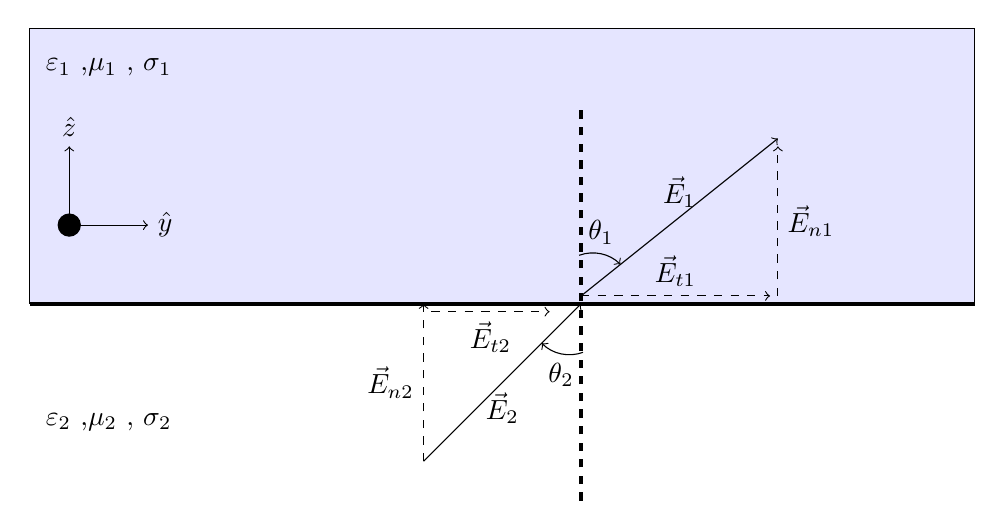
\begin{tikzpicture}

	\draw[fill=blue!10!white] (0,0) rectangle (12,3.5);
	\draw[ultra thick, black] (0,0) --++ (12,0);
	\node at (1,3) {$\varepsilon_1$ ,$\mu_1$ , $\sigma_1 $};
	\node at (1,-1.5) {$\varepsilon_2$ ,$\mu_2$ , $\sigma_2$};
	
	\draw[->] (0.5,1) --++ (1,0) node[right] {$\hat{y}$};
	\draw[->] (0.5,1) --++ (0,1) node[above] {$\hat{z}$};
	\draw[black, fill=black] (0.5,1) circle (4pt);
	
	% material 2
	\draw[->] (5,-2) --++ (2,2) node[midway, below] {$\vec{E}_2$}; 
	\draw[->, dashed] (5,-2) --++ (0,2) node[left, midway] {$\vec{E}_{\text{n2}}$};
	\draw[->, dashed] (5.1,-0.1) --++ (1.5,0) node[below, midway] {$\vec{E}_{\text{t2}}$};
	
	% material 1
	\draw[->] (7, 0.1)  --++ (2.5,2) node[midway, above] {$\vec{E}_{1}$};
	\draw[->, dashed] (9.5, 0.1) --++ (0,1.9) node[right, midway] {$\vec{E}_{\text{n1}}$};
	\draw[->, dashed] (7,0.1) --++ (2.4,0) node[above, midway] {$\vec{E}_{\text{t1}}$};
	
	
	
	% plane of incidence
	\draw[dashed, ultra thick] (7,-2.5) --++ (0,5); 
	\draw[<-] (7.5,0.5) arc (45:110:0.5) node[midway, above] {$\theta_1$};
	\draw[<-] (6.5,-0.5) arc (225:290:0.5) node[midway, below] {$\theta_2$};
	
\end{tikzpicture}
} % end scalebox
\end{textblock}
\begin{textblock}{5}(10,6)
\alert{
\begin{small}
\eq{
	&\text{Transverse} \longrightarrow  \\%\xhat, \yhat\\
	&\text{Normal} \longrightarrow \\%\zhat \\
	} % end eq
\end{small}
	} % end alert
\end{textblock}
\end{frame}

%%%%%%%%%%%%%%%%%%%%%%%%%%%%%%%%%%%%%%%%%%%%%%%%%%%%%%%%%%%%%%%
%%%%%%%%%%%%%%%%%%%%%%%%%%%%%%%%%%%%%%%%%%%%%%%%%%%%%%%%%%%%%%%
\begin{frame}{Your Turn: Example \#2}
\begin{textblock}{14.5}(0.5,4)

\end{textblock}
\end{frame}

%%%%%%%%%%%%%%%%%%%%%%%%%%%%%%%%%%%%%%%%%%%%%%%%%%%%%%%%%%%%%%%
%%%%%%%%%%%%%%%%%%%%%%%%%%%%%%%%%%%%%%%%%%%%%%%%%%%%%%%%%%%%%%%
\begin{frame}{Perfect Electric Conductors (PEC)}
\begin{textblock}{14.5}(0.5,2)
\begin{center}
\scalebox{0.75}{
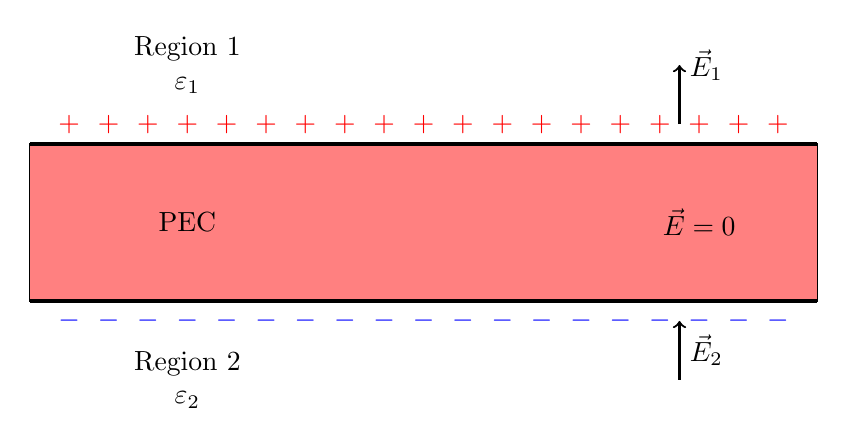
\begin{tikzpicture}
	\draw[fill=red!50!white] (0,0) rectangle ++(10,2); % PEC
	\draw[ultra thick] (0,0) --++(10,0); % lower PEC boundary
	\foreach \x in {0.5,1,...,9.5}{
		\node[blue] at (\x,-0.25) {$-$}; 
	} % lower boundary charges
	\draw[ultra thick] (0,2) --++(10,0); % upper PEC boundary
	\foreach \x in {0.5,1,...,9.5}{
		\node[red] at (\x,2.25) {$+$}; 
	} % upper boundary charges
	
	% material labels 
	\node[align=center] at (2,3) {Region 1 \\ $\varepsilon_1$};
	\node at (2,1) {PEC};
	\node[align=center] at (2,-1) {Region 2 \\ $\varepsilon_2$};
	
	% electric fields
	\draw[->, thick] (8.25,-1) --++ (0,0.75) node[midway, right] {$\vec{E}_2$};
	\node at (8.5,1) {$\vec{E} = 0$};
	\draw[->, thick] (8.25,2.25) --++ (0,0.75) node[right] {$\vec{E}_1$};
\end{tikzpicture}
} % end scalebox
\end{center}
\vspace{-12pt}
\begin{myblock}[0.9]{Electric Field in a PEC}
	\begin{enumerate}
		\item $\vec{E} = 0 $ inside a PEC 
		\item If $\vec{E}_{\text{PEC}} = 0$, then $\vec{E}_{\text{t,outside}} = \vec{E}_{\text{t,PEC}} = 0$
		\item Normal BC requires $\vec{E}_{\text{n, outside}} = \dfrac{\rho_S}{\varepsilon}$
		\item No static charge \textbf{inside} PEC  
	\end{enumerate}
\end{myblock}


\end{textblock}
\end{frame}

%%%%%%%%%%%%%%%%%%%%%%%%%%%%%%%%%%%%%%%%%%%%%%%%%%%%%%%%%%%%%%%
%%%%%%%%%%%%%%%%%%%%%%%%%%%%%%%%%%%%%%%%%%%%%%%%%%%%%%%%%%%%%%%
\begin{frame}{Capacitance}
\begin{textblock}{14.5}(0.5,2.5)
\begin{myblock}[0.9]{Capacitance}
\begin{enumerate}
	\item Capacitance is the ability of a structure to store energy in an electric field $\longrightarrow C = \dfrac{Q}{V}$
	\item Depends on the geometry and permittivity of medium separating plates.
\end{enumerate}
\end{myblock}
\vspace{-12pt}
\begin{small}
\alert{
\eq{
	Q (t) & = \int_{t_0}^t I(\tau) d\tau + Q (t_0) \\
	\implies V (t) &= \dfrac{1}{C}\int_{t_0}^t I(\tau) d\tau + \dfrac{1}{C}Q (t_0) 					= \dfrac{1}{C}\int_{t_0}^t I(\tau) d\tau + V_0 \\
	\implies I(t) &= C\partd{}{t} V(t)
} % end eq
} % end alert
\end{small}
\end{textblock}
\end{frame}


%%%%%%%%%%%%%%%%%%%%%%%%%%%%%%%%%%%%%%%%%%%%%%%%%%%%%%%%%%%%%%%
%%%%%%%%%%%%%%%%%%%%%%%%%%%%%%%%%%%%%%%%%%%%%%%%%%%%%%%%%%%%%%%
\begin{frame}{Parallel Plate Capacitor}
\begin{textblock}{8}(0.5,2.5)
\begin{center}
\begin{circuitikz}[scale=1]
	% 
	\draw[->] (6,0.75) --++ (0.75,0) node[right] {$\rho$}; 
	\draw[->] (6,0.75) --++ (0,0.75) node[above] {$z$};
	\draw (0,0) to[battery,a^=\myv{0}, invert] ++(0,3)
					to[short] ++(3,0)
					to[short] ++(0,-0.75)
					to[open] ++(0,-1.5)
					to[short] ++(0,-0.75)
					to[short] ++(-3,0);
	\node[ground] at (1.5,0){};
	% draw the capacitor
	\fill[pattern=north west lines, pattern color=gray!50!white] (1.25,0.75) rectangle (4.75,2.25);
	\draw[thick] (1.25,2.25) -- (4.75,2.25) node[right] {$z=d$}; % top wall
	\draw[thick] (1.25,0.75) -- (4.75,0.75) node[right] {$z=0$}; % bottom
	\foreach \x in {2,2.15,...,4}
	{
		\node at (\x,2.5){\tiny +};
		\node at (\x,0.5){\tiny -};
	}
\end{circuitikz}
\end{center}
\vspace{-12pt}
\begin{small}
\alert{
\eq{
	V &= -\int_C \vec{E} \mycdot d\ell \\
	&= -\int_0^d \dfrac{1}{\varepsilon} \vec{D} \mycdot \lp \zhat dz \rp\\
	&= -\int_0^d \lp -\zhat \dfrac{\rho_s}{\varepsilon} \rp \mycdot \lp \zhat dz \rp \\
	V &= - \dfrac{\rho_S d}{\varepsilon} 
} % end eq
} % end alert
\end{small}

\end{textblock}

\begin{textblock}{8}(8.5,9.5)
	\begin{small}
	\alert{
	Now the capacitance is:
	\eq{
		C &= \dfrac{Q}{V} = \dfrac{\rho_s A}{\frac{\rho_s d}{\varepsilon}} \\
		&= \dfrac{\varepsilon A}{d}
	} % end eq
	} % end alert
	\end{small}
\end{textblock}
\end{frame}

%%%%%%%%%%%%%%%%%%%%%%%%%%%%%%%%%%%%%%%%%%%%%%%%%%%%%%%%%%%%%%%
%%%%%%%%%%%%%%%%%%%%%%%%%%%%%%%%%%%%%%%%%%%%%%%%%%%%%%%%%%%%%%%
\begin{frame}{Coaxial Capacitor }
\begin{textblock}{8}(0.5,4)
Find the capacitance for a coaxial capacitor of length (in $z$-dimension) $\ell$. 
\scalebox{1}{
\begin{circuitikz}
\draw[pattern=north west lines, pattern color=gray!50!white] (0,0) circle (1.5);
\draw[black,fill=white] (0,0) circle (0.5);
\fill[black] (0,0) circle (1pt); % origin
\draw (120:0) -- node[right]{$b$}(120:1.5);
\draw (200:0) -- node[above]{$a$}(200:0.5);
%\draw[dashed, -stealth] (90:0) -- (90:2);
% \draw[red,-stealth] (0,1.75) arc (90:120:1.5) node[above,red]{$\phi$};
\draw (0:0.5) to[short] ++(2,0)
			to[battery, , a^=\myv{0}] ++(0,-2)
			to[short] ++(-2.25,0)
			to[short] ++(0,0.5);
\end{circuitikz}
} % end scalebox

\alert{
\eq{
	\vec{E} &= \rhohat \dfrac{\rho_\ell}{2\pi\varepsilon \rho} \\
	Q &= \rho_{\ell} \ell
}
}
\end{textblock}

\begin{textblock}{8}(8.5,3)
\begin{small}
\alert{
\eq{
	V &= -\int_C \vec{E}\mycdot \vec{d\ell} \\
	&= -\int_{\rho=a}^b \lp \rhohat \dfrac{\rho_\ell}{2\pi\varepsilon \rho} \rp \mycdot \lp \rhohat d\rho \rp \\
	&= -\dfrac{\rho_\ell}{2\pi\varepsilon} \int_{\rho=a}^b \dfrac{1}{\rho}d\rho \\
	&= \dfrac{\rho_\ell}{2\pi\varepsilon}  \text{ln}\lp \dfrac{b}{a} \rp \\
	\implies C&= \dfrac{Q}{V} = \dfrac{\rho_\ell \ell}{\frac{\rho_\ell}{2\pi\varepsilon}  \text{ln}\lp \dfrac{b}{a} \rp  } \\
	&= \dfrac{2\pi\varepsilon\ell}{ \text{ln}\lp \dfrac{b}{a} \rp }
} % end eq
} % end alert
\end{small}
\end{textblock}
\end{frame}

\end{lesson24}
\begin{lesson25}

\end{lesson25}